\chapter{The Riemann Integral} \label{int:chapter}

%%%%%%%%%%%%%%%%%%%%%%%%%%%%%%%%%%%%%%%%%%%%%%%%%%%%%%%%%%%%%%%%%%%%%%%%%%%%%%

\section{The Riemann integral}
\label{sec:rint}

\sectionnotes{1.5 lectures}

We now get to the fundamental concept of integration.  There is
often confusion among students of
calculus between \emph{integral} and \emph{antiderivative}.
The integral is (informally) the area under the curve, nothing else.
That we can compute an antiderivative using the integral is a nontrivial
result we have to prove.  
In this chapter we define the \emph{Riemann integral}%
\footnote{Named after the German mathematician
\href{https://en.wikipedia.org/wiki/Riemann}{Georg Friedrich Bernhard Riemann}
(1826--1866).}
using the Darboux integral%
\footnote{Named after the French mathematician
\href{https://en.wikipedia.org/wiki/Darboux}{Jean-Gaston Darboux} (1842--1917).},
which is technically simpler than (but equivalent to) the traditional
definition as done by Riemann.

\subsection{Partitions and lower and upper integrals}

We want to integrate a bounded function defined on an interval $[a,b]$.
We first define two auxiliary integrals that can be defined for all
bounded functions.  Only then can we talk about the Riemann integral and
the Riemann integrable functions.

\begin{defn}
A \emph{\myindex{partition}} $P$ of the interval $[a,b]$ is
a finite set of numbers $\{ x_0,x_1,x_2,\ldots,x_n \}$ such that
\begin{equation*}
a = x_0 < x_1 < x_2 < \cdots < x_{n-1} < x_n = b .
\end{equation*}
We write
\begin{equation*}
\Delta x_i := x_i - x_{i-1} .
\end{equation*}

\medskip

Let $f \colon [a,b] \to \R$ be a bounded function.  Let $P$ be a partition of
$[a,b]$.
Define
\begin{align*}
& m_i := \inf \, \bigl\{ f(x) : x_{i-1} \leq x \leq x_i \bigr\} , \\
& M_i := \sup \, \bigl\{ f(x) : x_{i-1} \leq x \leq x_i \bigr\} , \\
& L(P,f) :=
\sum_{i=1}^n m_i \Delta x_i , \\
& U(P,f) :=
\sum_{i=1}^n M_i \Delta x_i .
\end{align*}
We call $L(P,f)$ the \emph{\myindex{lower Darboux sum}} and
$U(P,f)$ the \emph{\myindex{upper Darboux sum}}\index{Darboux sum}.
\glsadd{not:lowerdarbouxsum}
\glsadd{not:upperdarbouxsum}
\end{defn}

The geometric idea of Darboux sums is indicated in
\figureref{darbouxfig}.  The lower sum is the area of the shaded
rectangles, and the upper sum is the area of the entire
rectangles, shaded plus unshaded parts.  The width of the $i$th rectangle is $\Delta x_i$,
the height of the shaded rectangle is $m_i$ and the height
of the entire rectangle is $M_i$.

\begin{myfigureht}
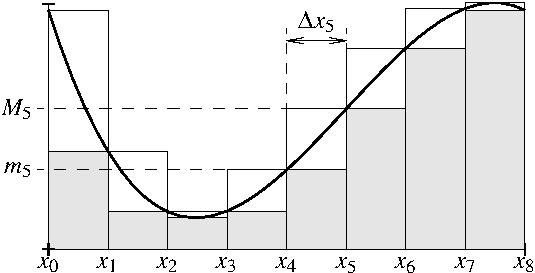
\includegraphics{figures/darbouxfig}
\caption{Sample Darboux sums.\label{darbouxfig}}
\end{myfigureht}

\begin{prop} \label{sumulbound:prop}
Let $f \colon [a,b] \to \R$ be a bounded function.  Let $m, M \in \R$ be 
such that for all $x$ we have $m \leq f(x) \leq M$.  For any partition $P$ of $[a,b]$
we have
\begin{equation}
\label{sumulbound:eq}
m(b-a) \leq
L(P,f) \leq U(P,f)
\leq M(b-a) .
\end{equation}
\end{prop}

\begin{proof}
Let $P$ be a partition.  Then note that $m \leq m_i$ for all $i$ and
$M_i \leq M$ for all $i$.  Also $m_i \leq M_i$ for all $i$.  Finally
$\sum_{i=1}^n \Delta x_i = (b-a)$.  Therefore,
\begin{multline*}
m(b-a) =
m \left( \sum_{i=1}^n \Delta x_i \right)
=
\sum_{i=1}^n m \Delta x_i
\leq
\sum_{i=1}^n m_i \Delta x_i 
\leq
\\
\leq
\sum_{i=1}^n M_i \Delta x_i
\leq
\sum_{i=1}^n M \Delta x_i 
=
M \left( \sum_{i=1}^n \Delta x_i \right)
=
M(b-a) .
\end{multline*}
Hence we get \eqref{sumulbound:eq}.  In particular, the set of lower and
upper sums are bounded sets.
\end{proof}

\begin{defn}
As the sets of lower and upper Darboux sums are bounded, we define
\begin{align*}
& \underline{\int_a^b} f(x)~dx :=
\sup \, \bigl\{ L(P,f) : P \text{ a partition of $[a,b]$} \bigr\} , \\
& \overline{\int_a^b} f(x)~dx :=
\inf \, \bigl\{ U(P,f) : P \text{ a partition of $[a,b]$} \bigr\} .
\end{align*}
We call $\underline{\int}$\glsadd{not:lowerdarboux}
the \emph{\myindex{lower Darboux integral}} and
$\overline{\int}$\glsadd{not:upperdarboux} the
\emph{\myindex{upper Darboux integral}}\index{Darboux integral}.
To avoid worrying about the variable of integration, 
we often simply write
\begin{equation*}
\underline{\int_a^b} f :=
\underline{\int_a^b} f(x)~dx 
\qquad \text{and} \qquad
\overline{\int_a^b} f :=
\overline{\int_a^b} f(x)~dx  .
\end{equation*}
\end{defn}

If integration is to make sense, then the lower and upper Darboux
integrals should be the same number, as we want a single number to call
\emph{the integral}.  However, these two integrals may in fact differ for
some functions.

\begin{example} \label{example:dirichletfunc}
Take the \myindex{Dirichlet function}
$f \colon [0,1] \to \R$, where $f(x) := 1$ if
$x \in \Q$ and $f(x) := 0$ if $x \notin \Q$.  Then
\begin{equation*}
\underline{\int_0^1} f = 0 \qquad \text{and} \qquad
\overline{\int_0^1} f = 1 .
\end{equation*}
The reason is that for every $i$ we have 
$m_i = \inf \{ f(x) : x \in [x_{i-1},x_i] \} = 0$  and
$M_i = \sup \{ f(x) : x \in [x_{i-1},x_i] \} = 1$.  Thus
\begin{align*}
& L(P,f) = \sum_{i=1}^n 0 \cdot \Delta x_i = 0 , \\
& U(P,f) = \sum_{i=1}^n 1 \cdot \Delta x_i = \sum_{i=1}^n \Delta x_i = 1  .
\end{align*}
\end{example}

\begin{remark}
The same definition of $\underline{\int_a^b} f$ and
$\overline{\int_a^b} f$
is used when $f$ is defined on a larger set $S$ such that
$[a,b] \subset S$.  In that case, we use the restriction of $f$ to $[a,b]$
and we must ensure that the restriction is bounded on $[a,b]$.
\end{remark}

To compute the integral we often take a partition $P$ and make it finer.
That is, we cut intervals in the partition into yet smaller pieces.

\begin{defn}
Let $P := \{ x_0, x_1, \ldots, x_n \}$ and
$\widetilde{P} := \{ \widetilde{x}_0, \widetilde{x}_1, \ldots, \widetilde{x}_m \}$ be
partitions of $[a,b]$.  We say $\widetilde{P}$ is a
\emph{refinement}\index{refinement of a partition} of $P$
if as sets $P \subset \widetilde{P}$.
\end{defn}

That is, $\widetilde{P}$ is a refinement of a partition if it contains all the
numbers in $P$ and perhaps some other numbers in between.  For example,
$\{ 0, 0.5, 1, 2 \}$ is a partition of $[0,2]$ and
$\{ 0, 0.2, 0.5, 1, 1.5, 1.75, 2 \}$ is a refinement.
The main reason for introducing refinements is the following proposition.

\begin{prop} \label{prop:refinement}
Let $f \colon [a,b] \to \R$ be a bounded function, and let $P$
be a partition of $[a,b]$.  Let $\widetilde{P}$ be a refinement of $P$.
Then
\begin{equation*}
L(P,f) \leq L(\widetilde{P},f) 
\qquad \text{and} \qquad
U(\widetilde{P},f) \leq U(P,f) .
\end{equation*}
\end{prop}

\begin{proof}
The tricky part of this proof is to get the notation correct.
Let $\widetilde{P} := \{ \widetilde{x}_0, \widetilde{x}_1, \ldots,
\widetilde{x}_m \}$ be
a refinement of 
$P := \{ x_0, x_1, \ldots, x_n \}$.  Then
$x_0 = \widetilde{x}_0$ and 
$x_n = \widetilde{x}_m$.  In fact, we can find integers
$k_0 < k_1 < \cdots < k_n$ such that $x_j = \widetilde{x}_{k_j}$ for
$j=0,1,2,\ldots,n$.

Let $\Delta \widetilde{x}_p = \widetilde{x}_p - \widetilde{x}_{p-1}$.
See \figureref{fig:refinement}.
We get 
\begin{equation*}
\Delta x_j
=
x_j - x_{j-1} =
\widetilde{x}_{k_j} - \widetilde{x}_{k_{j-1}} =
\sum_{p=k_{j-1}+1}^{k_j} 
\widetilde{x}_{p} - \widetilde{x}_{p-1}
=
\sum_{p=k_{j-1}+1}^{k_j} \Delta \widetilde{x}_p .
\end{equation*}
\begin{myfigureht}
\subimport*{figures/}{figrefinement.pdf_t}
\caption{Refinement of a subinterval.  Notice $\Delta x_j =
\Delta \widetilde{x}_{p-2} +
\Delta \widetilde{x}_{p-1} +
\Delta \widetilde{x}_{p}$,
and also
$k_{j-1}+1 = p-2$ and
$k_{j} = p$.\label{fig:refinement}}
\end{myfigureht}

Let $m_j$ be as before and correspond to the partition $P$.
Let $\widetilde{m}_j := \inf \{ f(x) : \widetilde{x}_{j-1} \leq x \leq
\widetilde{x}_j \}$.
Now, $m_j \leq \widetilde{m}_p$ for $k_{j-1} < p \leq k_j$.  Therefore,
\begin{equation*}
m_j \Delta x_j
=
m_j \sum_{p=k_{j-1}+1}^{k_j} \Delta \widetilde{x}_p
=
\sum_{p=k_{j-1}+1}^{k_j} m_j \Delta \widetilde{x}_p
\leq
\sum_{p=k_{j-1}+1}^{k_j} \widetilde{m}_p \Delta \widetilde{x}_p .
\end{equation*}
So
\begin{equation*}
L(P,f) =
\sum_{j=1}^n m_j \Delta x_j
\leq
\sum_{j=1}^n \,
\sum_{p=k_{j-1}+1}^{k_j} \widetilde{m}_p \Delta \widetilde{x}_p
=
\sum_{j=1}^m
\widetilde{m}_j \Delta \widetilde{x}_j = L(\widetilde{P},f).
\end{equation*}

The proof of $U(\widetilde{P},f) \leq U(P,f)$ is left as an exercise.
\end{proof}

Armed with refinements we prove the following.
The key point of this next proposition is that
the lower Darboux integral is less than or equal to the upper Darboux
integral.

\begin{prop} \label{intulbound:prop}
Let $f \colon [a,b] \to \R$ be a bounded function.  Let $m, M \in \R$ be 
such that for all $x \in [a,b]$ we have $m \leq f(x) \leq M$.  Then
\begin{equation}
\label{intulbound:eq}
m(b-a) \leq
\underline{\int_a^b} f \leq \overline{\int_a^b} f
\leq M(b-a) .
\end{equation}
\end{prop}

\begin{proof}
By \propref{sumulbound:prop} we have for any partition $P$
\begin{equation*}
m(b-a) \leq L(P,f) \leq U(P,f) \leq M(b-a).
\end{equation*}
The inequality
$m(b-a) \leq L(P,f)$ implies $m(b-a) \leq \underline{\int_a^b} f$.
Also
$U(P,f) \leq M(b-a)$ implies $\overline{\int_a^b} f \leq M(b-a)$.

The middle inequality in
\eqref{intulbound:eq} is the main point of this proposition.
Let $P_1, P_2$ be partitions of $[a,b]$.  Define 
$\widetilde{P} := P_1 \cup P_2$.
The set $\widetilde{P}$ is a partition of $[a,b]$, which
is a refinement of $P_1$ and a refinement of $P_2$.
By \propref{prop:refinement},
$L(P_1,f) \leq L(\widetilde{P},f)$ and
$U(\widetilde{P},f) \leq U(P_2,f)$.  So
\begin{equation*}
L(P_1,f) \leq L(\widetilde{P},f) \leq U(\widetilde{P},f) \leq U(P_2,f) .
\end{equation*}
In other words, for two arbitrary partitions $P_1$ and $P_2$, we have
$L(P_1,f) \leq U(P_2,f)$.  
Recall \propref{infsupineq:prop}, and take the supremum and
infimum over all partitions:
\begin{equation*}
\underline{\int_a^b} f = 
\sup \, \bigl\{ L(P,f) : \text{$P$ a partition of $[a,b]$} \bigr\}
\leq
\inf \, \bigl\{ U(P,f) : \text{$P$ a partition of $[a,b]$} \bigr\}
=
\overline{\int_a^b} f . \qedhere
\end{equation*}
\end{proof}

\subsection{Riemann integral}

We can finally define the Riemann integral.  However, the Riemann
integral is only defined on a certain class of functions, called the
Riemann integrable functions.

\begin{defn}
Let $f \colon [a,b] \to \R$ be a bounded function such that
\begin{equation*}
\underline{\int_a^b} f(x)~dx = \overline{\int_a^b} f(x)~dx .
\end{equation*}
Then $f$ is said to be \emph{\myindex{Riemann integrable}}.
The set of Riemann integrable functions on $[a,b]$ is denoted
by $\sR[a,b]$.\glsadd{not:integrablefunc}
When $f \in \sR[a,b]$ we define\glsadd{not:riemannint}
\begin{equation*}
\int_a^b f(x)~dx := 
\underline{\int_a^b} f(x)~dx = \overline{\int_a^b} f(x)~dx .
\end{equation*}
As before, we often simply write
\begin{equation*}
\int_a^b f := \int_a^b f(x)~dx.
\end{equation*}
The number $\int_a^b f$ is called the \emph{\myindex{Riemann integral}}
of $f$, or sometimes simply the \emph{integral} of $f$.
\end{defn}

By definition, any Riemann integrable function is bounded.
By appealing to \propref{intulbound:prop} we immediately obtain
the following proposition.  See also \figureref{fig:integralminmax}.

\begin{prop} \label{intbound:prop}
Let $f \colon [a,b] \to \R$ be a Riemann integrable function.
Let $m, M \in \R$ be 
such that $m \leq f(x) \leq M$ for all $x \in [a,b]$.  Then
\begin{equation*}
m(b-a) \leq
\int_a^b f
\leq M(b-a) .
\end{equation*}
\end{prop}
\begin{myfigureht}
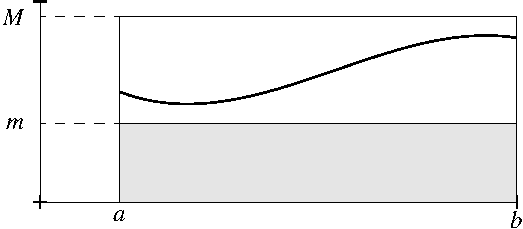
\includegraphics{figures/integralminmax}
\caption{The area under the curve is bounded from above by
the area of the entire rectangle, $M(b-a)$, and from below by
the area of the shaded part, $m(b-a)$.\label{fig:integralminmax}}
\end{myfigureht}

Often we use a weaker form of this proposition.  That is, if
$\abs{f(x)} \leq M$ for all $x \in [a,b]$, then
\begin{equation*}
\abs{\int_a^b f} \leq M(b-a) .
\end{equation*}

\begin{example}
We integrate constant functions using
\propref{intulbound:prop}.
If $f(x) := c$ for some constant $c$, then we take $m = M = c$.
In inequality \eqref{intulbound:eq}
all the inequalities must be equalities.
Thus $f$ is integrable on $[a,b]$ and $\int_a^b f = c(b-a)$.
\end{example}

\begin{example}
Let $f \colon [0,2] \to \R$ be defined by
\begin{equation*}
f(x) :=
\begin{cases}
1 & \text{ if $x < 1$,}\\
\nicefrac{1}{2} & \text{ if $x = 1$,}\\
0 & \text{ if $x > 1$.}
\end{cases}
\end{equation*}
We claim $f$ is Riemann integrable and $\int_0^2 f = 1$.

Proof: Let $0 < \epsilon < 1$ be arbitrary.
Let $P := \{0, 1-\epsilon, 1+\epsilon, 2\}$ be a partition.  We use the notation from
the definition of the Darboux sums.  Then
\begin{align*}
m_1 &= \inf \, \bigl\{ f(x) : x \in [0,1-\epsilon] \bigr\} = 1 , & 
M_1 &= \sup \, \bigl\{ f(x) : x \in [0,1-\epsilon] \bigr\} = 1 , \\
m_2 &= \inf \, \bigl\{ f(x) : x \in [1-\epsilon,1+\epsilon] \bigr\} = 0 , & 
M_2 &= \sup \, \bigl\{ f(x) : x \in [1-\epsilon,1+\epsilon] \bigr\} = 1 , \\
m_3 &= \inf \, \bigl\{ f(x) : x \in [1+\epsilon,2] \bigr\} = 0 , & 
M_3 &= \sup \, \bigl\{ f(x) : x \in [1+\epsilon,2] \bigr\} = 0 .
\end{align*}
Furthermore, $\Delta x_1 = 1-\epsilon$, $\Delta x_2 = 2\epsilon$ and
$\Delta x_3 = 1-\epsilon$.
See \figureref{darbouxfigstep}.
\begin{myfigureht}
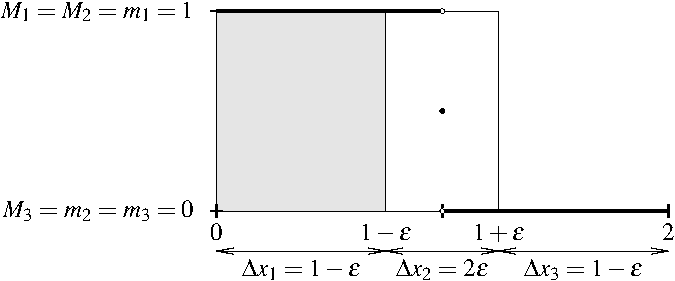
\includegraphics{figures/darbouxfigstep}
\caption{Darboux sums for the step function.  $L(P,f)$ is the area of the
shaded rectangle, $U(P,f)$ is the area of both rectangles, and
$U(P,f)-L(P,f)$ is the area of the unshaded rectangle.\label{darbouxfigstep}}
\end{myfigureht}

We compute
\begin{align*}
& L(P,f) = \sum_{i=1}^3 m_i \Delta x_i =
1 \cdot (1-\epsilon) + 0 \cdot 2\epsilon + 0 \cdot (1-\epsilon)
= 1-\epsilon , \\
& U(P,f) = \sum_{i=1}^3 M_i \Delta x_i =
1 \cdot (1-\epsilon) + 1 \cdot 2\epsilon + 0 \cdot (1-\epsilon)
= 1+\epsilon .
\end{align*}
Thus,
\begin{equation*}
\overline{\int_0^2} f - 
\underline{\int_0^2} f
\leq
U(P,f) - L(P,f)
=
(1+\epsilon)
- (1-\epsilon) = 2 \epsilon .
\end{equation*}
By \propref{intulbound:prop} we have $\underline{\int_0^2} f \leq \overline{\int_0^2} f$.
As $\epsilon$ was arbitrary we see 
$\overline{\int_0^2} f = \underline{\int_0^2} f$.  So $f$ is Riemann
integrable.  Finally,
\begin{equation*}
1-\epsilon = L(P,f) \leq \int_0^2 f \leq U(P,f) =
1+\epsilon.
\end{equation*}
Hence, $\bigl\lvert \int_0^2 f - 1 \bigr\rvert \leq \epsilon$.  As $\epsilon$ was arbitrary,
we have $\int_0^2 f = 1$.
\end{example}

It may be worthwhile to extract part of the technique of the example into a
proposition.

\begin{prop}
Let $f \colon [a,b] \to \R$ be a bounded function.  Then $f$ is Riemann
integrable if for every $\epsilon > 0$, there exists a partition $P$ such that
\begin{equation*}
U(P,f) - L(P,f) < \epsilon .
\end{equation*}
\end{prop}

\begin{proof}
If for every $\epsilon > 0$ such a $P$ exists, then we have:
\begin{equation*}
0 \leq
\overline{\int_a^b} f - 
\underline{\int_a^b} f
\leq
U(P,f) - L(P,f) < \epsilon .
\end{equation*}
Therefore, 
$\overline{\int_a^b} f = \underline{\int_a^b} f$, and $f$ is integrable.
\end{proof}

\begin{example}
Let us show $\frac{1}{1+x}$ is integrable on $[0,b]$ for any $b > 0$.
We will see later that all continuous functions are integrable, but let us
demonstrate how we do it directly.

Let $\epsilon > 0$ be given.  Take $n \in \N$ and
pick $x_j := \nicefrac{jb}{n}$, to form the 
partition $P := \{ x_0,x_1,\ldots,x_n \}$ of $[0,b]$.
We have $\Delta x_j = \nicefrac{b}{n}$ for all $j$.  
As $f$ is decreasing, for any subinterval $[x_{j-1},x_j]$ we obtain
\begin{equation*}
m_j = \inf \left\{ \frac{1}{1+x} : x \in [x_{j-1},x_j] \right\} = \frac{1}{1+x_j} ,
\qquad
M_j = \sup \left\{ \frac{1}{1+x} : x \in [x_{j-1},x_j] \right\} =
\frac{1}{1+x_{j-1}} .
\end{equation*}
Then we have
\begin{multline*}
U(P,f)-L(P,f)
=
\sum_{j=1}^n
\Delta x_j
(M_j-m_j)
=
\frac{b}{n}
\sum_{j=1}^n 
\left( \frac{1}{1+\nicefrac{(j-1)b}{n}} - \frac{1}{1+\nicefrac{jb}{n}} \right) 
=
\\
=
\frac{b}{n}
\left( \frac{1}{1+\nicefrac{0b}{n}} - \frac{1}{1+\nicefrac{nb}{n}} \right) 
=
\frac{b^2}{n(b+1)} .
\end{multline*}
The sum telescopes, the terms successively cancel each other, something
we have seen before.
Picking $n$ to be such that
$\frac{b^2}{n(b+1)} < \epsilon$ the proposition is satisfied, and the
function is integrable.
\end{example}

\subsection{More notation}

When $f \colon S \to \R$ is defined on a larger set $S$ and
$[a,b] \subset S$,
we say $f$ is Riemann integrable on $[a,b]$ if the restriction of $f$
to $[a,b]$ is Riemann integrable. 
In this case,
we say $f \in \sR[a,b]$,
and
we write $\int_a^b f$ to mean the Riemann integral
of the restriction of $f$ to $[a,b]$.

It is useful to define the integral $\int_a^b f$ even if
$a \not< b$.  Suppose $b < a$ and $f \in \sR[b,a]$,
then define
\begin{equation*}
\int_a^b f := - \int_b^a f .
\end{equation*}
For any function $f$ we define
\begin{equation*}
\int_a^a f := 0 .
\end{equation*}

At times, the variable $x$ may already have some other meaning.  When
we need to write down the variable of integration, we may simply
use a different letter.  For example,
\begin{equation*}
\int_a^b f(s)~ds := \int_a^b f(x)~dx .
\end{equation*}

\subsection{Exercises}

\begin{exercise}
Let $f \colon [0,1] \to \R$ be defined by $f(x) := x^3$
and let $P := \{ 0, 0.1, 0.4, 1 \}$.  Compute $L(P,f)$ and $U(P,f)$.
\end{exercise}

\begin{exercise}
Let $f \colon [0,1] \to \R$ be defined by $f(x) := x$.
Show that $f \in \sR[0,1]$ and
compute $\int_0^1 f$ using the definition of the integral
(but
feel free to use the propositions of this section).%\propref{intulbound:prop}).
\end{exercise}

\begin{exercise}
Let $f \colon [a,b] \to \R$ be a bounded function.
Suppose there exists a sequence of partitions $\{ P_k \}$ of $[a,b]$
such that
\begin{equation*}
\lim_{k \to \infty} \bigl( U(P_k,f) - L(P_k,f) \bigr) = 0 .
\end{equation*}
Show that $f$ is Riemann integrable and that
\begin{equation*}
\int_a^b f = 
\lim_{k \to \infty} U(P_k,f)
=
\lim_{k \to \infty} L(P_k,f) .
\end{equation*}
\end{exercise}

\begin{exercise}
Finish the proof of \propref{prop:refinement}.
\end{exercise}

\begin{exercise}
Suppose $f \colon [-1,1] \to \R$ is defined as
\begin{equation*}
f(x) :=
\begin{cases}
1 & \text{ if $x > 0$,} \\
0 & \text{ if $x \leq 0$.}
\end{cases}
\end{equation*}
Prove that $f \in \sR[-1,1]$ and
compute $\int_{-1}^1 f$ using the definition of the integral
(but
feel free to use the propositions of this section).
%(feel free to use \propref{intulbound:prop}).
\end{exercise}

\begin{exercise}
Let $c \in (a,b)$ and let $d \in \R$.
Define $f \colon [a,b] \to \R$ as
\begin{equation*}
f(x) :=
\begin{cases}
d & \text{ if $x = c$,} \\
0 & \text{ if $x \not= c$.}
\end{cases}
\end{equation*}
Prove that $f \in \sR[a,b]$ and
compute
$\int_a^b f$ using the definition of the integral
%(feel free to use \propref{intulbound:prop}).
(but
feel free to use the propositions of this section).
\end{exercise}

\begin{exercise} \label{exercise:taggedpartition}
Suppose $f \colon [a,b] \to \R$ is Riemann integrable.  Let $\epsilon
> 0$ be given.  Then show that there exists a partition $P = \{ x_0, x_1,
\ldots, x_n \}$
such that if we
pick any set of numbers $\{ c_1, c_2, \ldots, c_n \}$ with
$c_k \in [x_{k-1},x_k]$ for all $k$, then
\begin{equation*}
\abs{\int_a^b f - \sum_{k=1}^n f(c_k) \Delta x_k} < \epsilon .
\end{equation*}
\end{exercise}

\begin{exercise}
Let $f \colon [a,b] \to \R$ be a Riemann integrable function.
Let $\alpha > 0$ and $\beta \in \R$.
Then define $g(x) := f(\alpha x + \beta)$ on the interval
$I = [\frac{a-\beta}{\alpha}, \frac{b-\beta}{\alpha}]$.  Show
that $g$ is Riemann integrable on $I$.
\end{exercise}

\begin{exercise}
Suppose $f \colon [0,1] \to \R$ and $g \colon [0,1] \to \R$
are such that for all $x \in (0,1]$
we have $f(x) = g(x)$.  Suppose $f$ is Riemann integrable. 
Prove $g$ is Riemann integrable and $\int_{0}^1 f = \int_{0}^1 g$.
\end{exercise}

\begin{exercise}
Let $f \colon [0,1] \to \R$ be a bounded function.
Let $P_n = \{ x_0,x_1,\ldots,x_n \}$ be a uniform partition of $[0,1]$,
that is, $x_j := \nicefrac{j}{n}$.  Is $\{ L(P_n,f) \}_{n=1}^\infty$
always monotone?  Yes/No: Prove or find a counterexample.
\end{exercise}

\begin{exercise}[Challenging]
For a bounded function $f \colon [0,1] \to \R$ let
$R_n := (\nicefrac{1}{n})\sum_{j=1}^n f(\nicefrac{j}{n})$ (the
uniform right hand rule).
\begin{enumerate}[a)]
\item
If $f$ is Riemann integrable show $\int_0^1 f = \lim \, R_n$.
\item
Find an $f$ that is not Riemann integrable, but $\lim \, R_n$ exists.
\end{enumerate}
\end{exercise}

\begin{exercise}[Challenging] \label{exercise:riemannintdarboux}
Generalize the previous exercise.
Show that $f \in \sR[a,b]$ if and only if there exists an $I \in \R$,
such that for every $\epsilon > 0$ there exists
a $\delta > 0$ such that if $P$ is a partition with $\Delta x_i < \delta$
for all $i$, then
$\abs{L(P,f) - I} < \epsilon$ and
$\abs{U(P,f) - I} < \epsilon$.  If $f \in \sR[a,b]$, then $I = \int_a^b f$.
\end{exercise}

\begin{exercise}
Using \exerciseref{exercise:riemannintdarboux} and the idea of
the proof in \exerciseref{exercise:taggedpartition}, show that 
Darboux integral is the same as the standard definition
of Riemann integral, which you have most likely seen in calculus.  That is,
show that
$f \in \sR[a,b]$ if and only if there exists an $I \in \R$,
such that for every $\epsilon > 0$ there exists
a $\delta > 0$ such that if $P = \{ x_0,x_1,\ldots,x_n \}$
is a partition with $\Delta x_i < \delta$
for all $i$, then
$\abs{\sum_{i=1}^n f(c_i) \Delta x_i - I} < \epsilon$ for any set
$\{ c_1,c_2,\ldots,c_n \}$ with $c_i \in [x_{i-1},x_i]$.
If $f \in \sR[a,b]$, then $I = \int_a^b f$.
\end{exercise}


\begin{exercise}[Challenging]
Construct functions $f$ and $g$, 
where
$f \colon [0,1] \to \R$ is Riemann integrable,
$g \colon [0,1] \to [0,1]$ is one-to-one and onto,
and such that the composition $f \circ g$ is not Riemann integrable.
\end{exercise}

%%%%%%%%%%%%%%%%%%%%%%%%%%%%%%%%%%%%%%%%%%%%%%%%%%%%%%%%%%%%%%%%%%%%%%%%%%%%%%

\sectionnewpage
\section{Properties of the integral}
\label{sec:rintprop}

\sectionnotes{2 lectures, integrability of functions with 
discontinuities can safely be skipped}

\subsection{Additivity}

The next result we prove is usually referred to as the
\myindex{additive property of the integral}.  First we prove the additivity
property for the lower and upper Darboux integrals.

\begin{lemma} \label{lemma:darbouxadd}
Suppose $a < b < c$ and $f \colon [a,c] \to \R$ is a bounded function.
Then
\begin{equation*}
\underline{\int_a^c} f
=
\underline{\int_a^b} f
+
\underline{\int_b^c} f
\end{equation*}
and
\begin{equation*}
\overline{\int_a^c} f
=
\overline{\int_a^b} f
+
\overline{\int_b^c} f .
\end{equation*}
\end{lemma}

\begin{proof}
If we have partitions $P_1 = \{ x_0,x_1,\ldots,x_k \}$
of $[a,b]$ and $P_2 = \{ x_k, x_{k+1}, \ldots, x_n \}$ of $[b,c]$,
then the set $P := P_1 \cup P_2 = \{ x_0, x_1, \ldots, x_n \}$ is
a partition of $[a,c]$.  Then
\begin{equation*}
L(P,f) =
\sum_{j=1}^n m_j \Delta x_j
=
\sum_{j=1}^k m_j \Delta x_j
+
\sum_{j=k+1}^n m_j \Delta x_j
=
L(P_1,f) + L(P_2,f) .
\end{equation*}
When we take the supremum of the right hand side over all $P_1$ and $P_2$,
we are taking a supremum of the left hand side
over all partitions $P$ of $[a,c]$ that contain $b$.  If $Q$ is any partition
of $[a,c]$ and $P = Q \cup \{ b \}$, then $P$ is a refinement of $Q$
and so $L(Q,f) \leq L(P,f)$.  Therefore, taking a supremum only over the $P$
that contain $b$ is sufficient to find the supremum of $L(P,f)$
over all partitions $P$, see \exerciseref{exercise:dominatingb}.
Finally recall \exerciseref{exercise:supofsum}
to compute
\begin{equation*}
\begin{split}
\underline{\int_a^c} f
& =
\sup \, \bigl\{ L(P,f) : \text{$P$ a partition of $[a,c]$} \bigr\}
\\
& =
\sup \, \bigl\{ L(P,f) : \text{$P$ a partition of $[a,c]$, $b \in P$} \bigr\}
\\
& =
\sup \, \bigl\{ L(P_1,f) + L(P_2,f) :
\text{$P_1$ a partition of $[a,b]$, $P_2$ a partition of $[b,c]$} \bigr\}
\\
& =
\sup \, \bigl\{ L(P_1,f) : \text{$P_1$ a partition of $[a,b]$} \bigr\}
+
\sup \, \bigl\{ L(P_2,f) : \text{$P_2$ a partition of $[b,c]$} \bigr\}
\\
&=
\underline{\int_a^b} f + \underline{\int_b^c} f .
\end{split}
\end{equation*}

Similarly, for $P$, $P_1$, and $P_2$ as above we obtain
\begin{equation*}
U(P,f) =
\sum_{j=1}^n M_j \Delta x_j
=
\sum_{j=1}^k M_j \Delta x_j
+
\sum_{j=k+1}^n M_j \Delta x_j
=
U(P_1,f) + U(P_2,f) .
\end{equation*}
We wish to take the infimum on the right
over all $P_1$ and $P_2$, and so we are taking the infimum
over all partitions $P$ of $[a,c]$ that contain $b$.  If $Q$ is any partition
of $[a,c]$ and $P = Q \cup \{ b \}$, then $P$ is a refinement of $Q$
and so $U(Q,f) \geq U(P,f)$.  Therefore, taking an infimum only over the $P$
that contain $b$ is sufficient to find the infimum of $U(P,f)$ for
all $P$.
We obtain
\begin{equation*}
\overline{\int_a^c} f
=
\overline{\int_a^b} f + \overline{\int_b^c} f .  \qedhere
\end{equation*}
\end{proof}

\begin{prop}
Let $a < b < c$.  A function $f \colon [a,c] \to \R$ is Riemann integrable
if and only if $f$ is Riemann integrable on $[a,b]$ and $[b,c]$.  If
$f$ is Riemann integrable, then
\begin{equation*}
\int_a^c f
=
\int_a^b f
+
\int_b^c f .
\end{equation*}
\end{prop}

\begin{proof}
Suppose $f \in \sR[a,c]$, then 
$\overline{\int_a^c} f = 
\underline{\int_a^c} f = 
\int_a^c f$.  We apply the lemma to get
\begin{equation*}
\int_a^c f
=
\underline{\int_a^c} f
 =
\underline{\int_a^b} f + \underline{\int_b^c} f
 \leq
\overline{\int_a^b} f + \overline{\int_b^c} f
 =
\overline{\int_a^c} f
 =
\int_a^c f .
\end{equation*}
Thus the inequality is an equality and
\begin{equation*}
\underline{\int_a^b} f + \underline{\int_b^c} f
=
\overline{\int_a^b} f + \overline{\int_b^c} f .
\end{equation*}
As we also know 
$\underline{\int_a^b} f \leq \overline{\int_a^b} f$
and
$\underline{\int_b^c} f \leq \overline{\int_b^c} f$, we 
conclude 
\begin{equation*}
\underline{\int_a^b} f
=
\overline{\int_a^b} f
\qquad \text{and} \qquad
\underline{\int_b^c} f
=
\overline{\int_b^c} f .
\end{equation*}
Thus $f$ is Riemann integrable on $[a,b]$ and $[b,c]$ and the desired formula
holds.

Now assume the restrictions of $f$ to $[a,b]$ and to $[b,c]$
are Riemann integrable.  We again apply the lemma to get
\begin{equation*}
\underline{\int_a^c} f
=
\underline{\int_a^b} f + \underline{\int_b^c} f
=
\int_a^b f + \int_b^c f
=
\overline{\int_a^b} f + \overline{\int_b^c} f
=
\overline{\int_a^c} f .
\end{equation*}
Therefore, $f$ is Riemann integrable on $[a,c]$, and the integral is computed
as indicated.
\end{proof}

An easy consequence of the additivity is the following corollary.  We
leave the details to the reader as an exercise.

\begin{cor} \label{intsubcor}
If $f \in \sR[a,b]$ and
$[c,d] \subset [a,b]$, then
the restriction $f|_{[c,d]}$ is in $\sR[c,d]$.
\end{cor}

\subsection{Linearity and monotonicity}

\begin{prop}[Linearity]
\index{linearity of the integral}
Let $f$ and $g$ be in $\sR[a,b]$ and $\alpha \in \R$.
\begin{enumerate}[(i)]
\item $\alpha f$ is in $\sR[a,b]$ and
\begin{equation*}
\int_a^b \alpha f(x) ~dx = \alpha \int_a^b f(x) ~dx .
\end{equation*}
\item $f+g$ is in $\sR[a,b]$ and
\begin{equation*}
\int_a^b \bigl( f(x)+g(x) \bigr) ~dx = 
\int_a^b f(x) ~dx 
+
\int_a^b g(x) ~dx .
\end{equation*}
\end{enumerate}
\end{prop}

\pagebreak[2]
\begin{proof}
Let us prove the first item for $\alpha \geq 0$. 
Let $P$ be a partition of $[a,b]$.
Let $m_i := \inf \{ f(x) : x \in [x_{i-1},x_i] \}$ as usual.
Since $\alpha$ is nonnegative, we can move the multiplication by $\alpha$
past the infimum,
\begin{equation*}
\inf \{ \alpha f(x) : x \in [x_{i-1},x_i] \}
=
\alpha \inf \{ f(x) : x \in [x_{i-1},x_i] \} = \alpha m_i .
\end{equation*}
Therefore
\begin{equation*}
L(P,\alpha f) =
\sum_{i=1}^n \alpha m_i \Delta_i = \alpha \sum_{i=1}^n m_i \Delta_i = \alpha
L(P,f).
\end{equation*}
Similarly,
\begin{equation*}
U(P,\alpha f) = \alpha U(P,f) .
\end{equation*}
Again, as $\alpha \geq 0$ we
may move multiplication by $\alpha$ past the supremum.  Hence,
\begin{equation*}
\begin{split}
\underline{\int_a^b} \alpha f(x)~dx & =
\sup \, \bigl\{ L(P,\alpha f) : \text{$P$ a partition of $[a,b]$} \bigr\}
\\
& =
\sup \, \bigl\{ \alpha L(P,f) : \text{$P$ a partition of $[a,b]$} \bigr\}
\\
& =
\alpha \,
\sup \, \bigl\{ L(P,f) : \text{$P$ a partition of $[a,b]$} \bigr\}
\\
& =
\alpha
\underline{\int_a^b} f(x)~dx .
\end{split}
\end{equation*}
Similarly, we show 
\begin{equation*}
\overline{\int_a^b} \alpha f(x)~dx
=
\alpha
\overline{\int_a^b} f(x)~dx .
\end{equation*}
The conclusion now follows for $\alpha \geq 0$.

To finish the proof of the first item, we need to show 
that $-f$ is Riemann integrable and
$\int_a^b - f(x)~dx =
-
\int_a^b f(x)~dx$.  The proof of this fact is left as an exercise.

The proof of the second item in the proposition is also left as an exercise.
It is not as
trivial as it may appear at first glance.
\end{proof}

The second item in the proposition does not hold with
equality for the Darboux integrals, but we do obtain inequalities.

\begin{prop} \label{prop:upperlowerlinineq}
Let $f \colon [a,b] \to \R$ and $g \colon [a,b] \to \R$ be bounded
functions.  Then
\begin{equation*}
%\overline{\int_a^b} \bigl(f(x)+g(x)\bigr)~dx \leq
%\overline{\int_a^b}f(x)~dx+\overline{\int_a^b}g(x)~dx
\overline{\int_a^b} (f+g) \leq \overline{\int_a^b}f+\overline{\int_a^b}g
,
\qquad
\text{and}
\qquad
\underline{\int_a^b} (f+g) \geq \underline{\int_a^b}f+\underline{\int_a^b}g
%\underline{\int_a^b} \bigl(f(x)+g(x)\bigr)~dx \geq
%\underline{\int_a^b}f(x)~dx+\underline{\int_a^b}g(x)~dx
.
\end{equation*}
\end{prop}

The proof of the above proposition is \exerciseref{exercise:upperlowerlinineq}.
It follows as supremum of a sum is less than or equal to the sum of
suprema and similarly for infima, see \exerciseref{exercise:sumofsup}.

\begin{prop}[Monotonicity]
\index{monotonicity of the integral}
Let $f \colon [a,b] \to \R$ and $g \colon [a,b] \to \R$ be
bounded, and $f(x) \leq g(x)$
for all $x \in [a,b]$.  Then
\begin{equation*}
\underline{\int_a^b} f 
\leq
\underline{\int_a^b} g 
\qquad \text{and} \qquad
\overline{\int_a^b} f 
\leq
\overline{\int_a^b} g .
\end{equation*}
Moreover, if $f$ and $g$ are in $\sR[a,b]$, then
\begin{equation*}
\int_a^b f 
\leq
\int_a^b g .
\end{equation*}
\end{prop}

\begin{proof}
Let $P = \{ x_0, x_1, \ldots, x_n \}$ be a partition of $[a,b]$.  Then
let
\begin{equation*}
m_i := \inf \, \bigl\{ f(x) : x \in [x_{i-1},x_i] \bigr\}
\qquad \text{and} \qquad
\widetilde{m}_i := \inf \, \bigl\{ g(x) : x \in [x_{i-1},x_i] \bigr\} .
\end{equation*}
As $f(x) \leq g(x)$, then $m_i \leq \widetilde{m}_i$.
Therefore,
\begin{equation*}
L(P,f)
=
\sum_{i=1}^n m_i \Delta x_i
\leq
\sum_{i=1}^n \widetilde{m}_i \Delta x_i
=
L(P,g) .
\end{equation*}
We take the supremum over all $P$ (see \propref{prop:funcsupinf}) to obtain 
\begin{equation*}
\underline{\int_a^b} f 
\leq
\underline{\int_a^b} g .
\end{equation*}
Similarly, we obtain the same conclusion for the upper integrals.
Finally,
if $f$ and $g$ are Riemann integrable all the integrals are equal,
and the conclusion follows.
\end{proof}

\subsection{Continuous functions}

Let us show that continuous functions are Riemann integrable.  In fact, we
will show we can even allow some discontinuities.  We start with a
function continuous on the whole closed interval $[a,b]$.

\begin{lemma} \label{lemma:contint}
If $f \colon [a,b] \to \R$ is a continuous function,
then $f \in \sR[a,b]$.
\end{lemma}

\begin{proof}
As $f$ is continuous on a closed bounded interval, it is
uniformly continuous.
Let $\epsilon > 0$ be given.  Find a $\delta > 0$ such that
$\abs{x-y} < \delta$ implies $\abs{f(x)-f(y)} < \frac{\epsilon}{b-a}$.

Let $P = \{ x_0, x_1, \ldots, x_n \}$
be a partition of $[a,b]$ such that $\Delta x_i < \delta$ for all $i = 1,2,
\ldots, n$.  For example,
take $n$ such that $\frac{b-a}{n} < \delta$ and
let $x_i := \frac{i}{n}(b-a) + a$.
Then for all $x, y \in [x_{i-1},x_i]$ we have 
$\abs{x-y} \leq \Delta x_i < \delta$ and so
\begin{equation*}
f(x)-f(y) \leq \abs{f(x)-f(y)} < \frac{\epsilon}{b-a} .
\end{equation*}
As $f$ is continuous on $[x_{i-1},x_i]$, it attains a maximum and a minimum
on this interval.
Let $x$ be a point where $f$ attains the maximum and $y$ be a point
where $f$ attains the minimum.  Then $f(x) = M_i$
and $f(y) = m_i$ in the notation from the definition of the integral.
Therefore,
\begin{equation*}
M_i-m_i = f(x)-f(y) < 
\frac{\epsilon}{b-a} .
\end{equation*}
And so
\begin{equation*}
\begin{split}
\overline{\int_a^b} f - 
\underline{\int_a^b} f 
& \leq
U(P,f) - L(P,f)
\\
& =
\left(
\sum_{i=1}^n
M_i \Delta x_i
\right)
-
\left(
\sum_{i=1}^n
m_i \Delta x_i
\right)
\\
& =
\sum_{i=1}^n
(M_i-m_i) \Delta x_i
\\
& <
\frac{\epsilon}{b-a}
\sum_{i=1}^n
\Delta x_i
\\
& =
\frac{\epsilon}{b-a} (b-a)
= \epsilon .
\end{split}
\end{equation*}
As $\epsilon > 0$ was arbitrary,
\begin{equation*}
\overline{\int_a^b} f = \underline{\int_a^b} f ,
\end{equation*}
and $f$ is Riemann integrable on $[a,b]$.
\end{proof}

The second lemma says that we need the function to only be ``Riemann integrable
inside the interval,'' as long as it is bounded.  It also tells us how to
compute the integral.

\begin{lemma} \label{lemma:boundedimpriemann}
Let $f \colon [a,b] \to \R$ be a bounded function,
$\{ a_n \}$ and $\{b_n \}$ be sequences such that
$a < a_n < b_n < b$ for all $n$, with
$\lim \, a_n = a$ and $\lim \, b_n = b$.
Suppose $f \in \sR[a_n,b_n]$ for all $n$.
Then $f \in \sR[a,b]$ and
\begin{equation*}
\int_a^b f = 
\lim_{n \to \infty} \int_{a_n}^{b_n} f .
\end{equation*}
\end{lemma}

\begin{proof}
Let $M > 0$ be a real number such that $\abs{f(x)} \leq M$.
As $(b-a) \geq (b_n-a_n)$,
\begin{equation*}
-M(b-a) \leq
-M(b_n-a_n) \leq
\int_{a_n}^{b_n} f
\leq
M(b_n-a_n) \leq
M(b-a) .
\end{equation*}
Therefore, the sequence of numbers
$\bigl\{ \int_{a_n}^{b_n} f \bigr\}_{n=1}^\infty$ is bounded and by
\hyperref[thm:bwseq]{Bolzano--Weierstrass}
has a convergent subsequence indexed by $n_k$.  Let us call
$L$ the limit of the subsequence
$\bigl\{ \int_{a_{n_k}}^{b_{n_k}} f \bigr\}_{k=1}^\infty$.

\lemmaref{lemma:darbouxadd} says that
the lower and upper integral are additive
and the hypothesis says that
$f$ is integrable on $[a_{n_k},b_{n_k}]$.
Therefore
\begin{equation*}
\underline{\int_a^b} f
=
\underline{\int_a^{a_{n_k}}} f
+
\int_{a_{n_k}}^{b_{n_k}} f
+
\underline{\int_{b_{n_k}}^b} f
\geq
-M(a_{n_k}-a)
+
\int_{a_{n_k}}^{b_{n_k}} f
-
M(b-b_{n_k}) .
\end{equation*}
We take the limit as $k$ goes to $\infty$ on the right-hand side,
\begin{equation*}
\underline{\int_a^b} f
\geq
-M\cdot 0
+
L
-
M\cdot 0
= L .
\end{equation*}

Next we use additivity of the upper integral,
\begin{equation*}
\overline{\int_a^b} f
=
\overline{\int_a^{a_{n_k}}} f
+
\int_{a_{n_k}}^{b_{n_k}} f
+
\overline{\int_{b_{n_k}}^b} f
\leq
M(a_{n_k}-a)
+
\int_{a_{n_k}}^{b_{n_k}} f
+
M(b-b_{n_k}) .
\end{equation*}
We take the same subsequence 
$\{ \int_{a_{n_k}}^{b_{n_k}} f \}_{k=1}^\infty$ and take the limit 
to obtain
\begin{equation*}
\overline{\int_a^b} f
\leq
M\cdot 0
+
L
+
M\cdot 0
= L .
\end{equation*}
Thus $\overline{\int_a^b} f = \underline{\int_a^b} f = L$
and hence $f$ is Riemann integrable and $\int_a^b f = L$.
In particular, no matter what
subsequence we chose,
the $L$ is the same number.

To prove the final statement of the lemma we use 
\propref{seqconvsubseqconv:prop}.  We have shown that every convergent
subsequence
$\bigl\{ \int_{a_{n_k}}^{b_{n_k}} f \bigr\}$ converges to $L = \int_a^b f$.
Therefore, the sequence
$\bigl\{ \int_{a_n}^{b_n} f \bigr\}$ is convergent and converges to $\int_a^b f$.
\end{proof}

We say a function $f \colon [a,b] \to \R$ has \emph{\myindex{finitely many
discontinuities}} if there exists a finite set $S := \{ x_1, x_2, \ldots, x_n \}
\subset [a,b]$, and $f$ is continuous
at all points of $[a,b] \setminus S$.

\begin{thm}
Let $f \colon [a,b] \to \R$ be a bounded function with finitely
many discontinuities.  Then $f \in \sR[a,b]$.
\end{thm}

\begin{proof}
We divide the interval into finitely many intervals $[a_i,b_i]$
so that $f$ is continuous
on the interior $(a_i,b_i)$.  If $f$ is continuous on $(a_i,b_i)$,
then it is continuous and hence integrable on $[c_i,d_i]$ whenever $a_i < c_i < d_i < b_i$.  By
\lemmaref{lemma:boundedimpriemann}
the restriction
of $f$ to $[a_i,b_i]$ is integrable.  By additivity of the integral (and
\hyperref[induction:thm]{induction}) $f$ is integrable on the union of the intervals.
\end{proof}

\subsection{More on integrable functions}

Sometimes it is convenient (or necessary)
to change certain values of a function and
then integrate.  The next result says
that if we change the values only at finitely
many points, the integral does not change.

\begin{prop}
Let $f \colon [a,b] \to \R$ be Riemann integrable.  Let $g \colon [a,b] \to
\R$ be a function such that $f(x) = g(x)$ for all $x \in [a,b] \setminus S$,
where $S$ is a finite set.  Then $g$ is a Riemann integrable function
and
\begin{equation*}
\int_a^b g = \int_a^b f.
\end{equation*}
\end{prop}

\begin{proof}[Sketch of proof]
Using additivity of the integral, we split up the interval $[a,b]$ into
smaller intervals such that $f(x) = g(x)$ holds for all $x$ except at the
endpoints (details are left to the reader).

Therefore, without loss of generality suppose $f(x) = g(x)$ for
all $x \in (a,b)$.  The proof follows by \lemmaref{lemma:boundedimpriemann},
and is left as an exercise.
\end{proof}

Finally, monotone (increasing or decreasing) functions are always
Riemann integrable.  The proof is left to the reader as
\exerciseref{exercise:boundedvariationintegrable}.

\begin{prop} \label{prop:monotoneintegrable}
Let $f \colon [a,b] \to \R$ be a monotone function.  Then $f \in \sR[a,b]$.
\end{prop}

\subsection{Exercises}

\begin{exercise}
Let $f$ be in $\sR[a,b]$.  Prove that
$-f$ is in $\sR[a,b]$ and 
\begin{equation*}
\int_a^b - f(x) ~dx = - \int_a^b f(x) ~dx .
\end{equation*}
\end{exercise}

\begin{exercise}
Let $f$ and $g$ be in $\sR[a,b]$.
Prove, without using \propref{prop:upperlowerlinineq}, that $f+g$ is in $\sR[a,b]$ and
\begin{equation*}
\int_a^b \bigl( f(x)+g(x) \bigr) ~dx = 
\int_a^b f(x) ~dx 
+
\int_a^b g(x) ~dx .
\end{equation*}
Hint: One way to do it is to use \propref{prop:refinement} to find a single partition $P$
such that $U(P,f)-L(P,f) < \nicefrac{\epsilon}{2}$ and
$U(P,g)-L(P,g) < \nicefrac{\epsilon}{2}$.
\end{exercise}

\begin{exercise}
Let $f \colon [a,b] \to \R$ be Riemann integrable.  Let $g \colon [a,b] \to
\R$ be a function such that $f(x) = g(x)$ for all $x \in (a,b)$.
Prove that $g$ is Riemann integrable and that
\begin{equation*}
\int_a^b g = \int_a^b f.
\end{equation*}
\end{exercise}

\begin{exercise}
Prove the \emph{\myindex{mean value theorem for integrals}}.  That is,
prove that if $f \colon [a,b] \to \R$ is continuous, then there exists
a $c \in [a,b]$ such that $\int_a^b f = f(c)(b-a)$.
\end{exercise}

\begin{exercise}
Let $f \colon [a,b] \to \R$ be a continuous function such that $f(x) \geq 0$
for all $x \in [a,b]$ and $\int_a^b f = 0$.  Prove that $f(x) = 0$
for all $x$.
\end{exercise}

\begin{exercise}
Let $f \colon [a,b] \to \R$ be a continuous function
and $\int_a^b f = 0$.  Prove that
there exists a $c \in [a,b]$ such that $f(c) = 0$ (Compare with the
previous exercise).
\end{exercise}

\begin{exercise}
Let $f \colon [a,b] \to \R$ and $g \colon [a,b] \to \R$
be continuous functions such that $\int_a^b f = \int_a^b g$.
Show that there exists a $c \in [a,b]$ such that $f(c) = g(c)$.
\end{exercise}

\begin{exercise}
Let $f \in \sR[a,b]$.  Let $\alpha, \beta, \gamma$ be arbitrary numbers in
$[a,b]$ (not necessarily ordered in any way).  Prove 
\begin{equation*}
\int_\alpha^\gamma f =
\int_\alpha^\beta f +
\int_\beta^\gamma f .
\end{equation*}
Recall what $\int_a^b f$ means if $b \leq a$.
\end{exercise}

\begin{exercise}
Prove \corref{intsubcor}.
\end{exercise}

\begin{exercise} \label{exercise:easyabsint}
Suppose $f \colon [a,b] \to \R$ is bounded and
has finitely many discontinuities.
Show that as a function of $x$ the expression $\abs{f(x)}$ is bounded with finitely many
discontinuities and is thus Riemann integrable.  Then show 
\begin{equation*}
\abs{\int_a^b f(x)~dx} \leq \int_a^b \abs{f(x)}~dx .
\end{equation*}
\end{exercise}

\begin{exercise}[Hard]
Show that the
Thomae\index{Thomae function} or \myindex{popcorn function}
(see \exampleref{popcornfunction:example})
is Riemann integrable.  Therefore, there exists a
function discontinuous at all rational numbers (a dense set)
that is Riemann integrable.

In particular,
define $f \colon [0,1] \to \R$ by
\begin{equation*}
f(x) := 
\begin{cases}
\nicefrac{1}{k} & \text{ if $x=\nicefrac{m}{k}$ where $m,k \in \N$
and $m$ and $k$ have no common divisors,} \\
0 & \text{ if $x$ is irrational}.
\end{cases}
\end{equation*}
Show $\int_0^1 f = 0$.
\end{exercise}


\begin{exnote}
If $I \subset \R$ is a bounded interval, then
the function
\begin{equation*}
\varphi_I(x) :=
\begin{cases}
1 & \text{if $x \in I$,} \\
0 & \text{otherwise,}
\end{cases}
\end{equation*}
is called an \emph{\myindex{elementary step function}}.
\end{exnote}

\begin{exercise}
Let $I$ be an arbitrary bounded interval (you should consider all types
of intervals: closed, open, half-open) and $a < b$, then
using only the definition of the integral
show that
the elementary step function $\varphi_I$ is integrable
on $[a,b]$, and find the integral in terms of $a$, $b$, and the
endpoints of $I$.
\end{exercise}

\begin{exnote}
When a function $f$ can be written as
\begin{equation*}
f(x) = \sum_{k=1}^n \alpha_k \varphi_{I_k} (x)
\end{equation*}
for some real numbers $\alpha_1,\alpha_2, \ldots, \alpha_n$
and some bounded intervals $I_1,I_2,\ldots,I_n$, then 
$f$ is called a \emph{\myindex{step function}}.
\end{exnote}

\begin{exercise}
Using the previous exercise, show that a step function is integrable
on any interval $[a,b]$.  Furthermore, find the integral in terms of
$a$, $b$, the endpoints of $I_k$ and the $\alpha_k$.
\end{exercise}

\begin{exercise}
\label{exercise:boundedvariationintegrable}
Let $f \colon [a,b] \to \R$ be increasing.
\begin{enumerate}[a)]
\item
Show that $f$ is Riemann
integrable.  Hint: Use a uniform partition; each subinterval of same length.
\item
Use part a to show that a decreasing function is Riemann
integrable.
\item
Suppose\footnote{Such an $h$ is said to be of \emph{\myindex{bounded variation}}.}
$h = f-g$ where $f$ and $g$ are increasing
functions on $[a,b]$.  Show that $h$ is Riemann integrable.
\end{enumerate}
\end{exercise}

\begin{exercise}[Challenging] \label{exercise:hardabsint}
Suppose $f \in \sR[a,b]$, then the function that takes $x$ to
$\abs{f(x)}$ is also Riemann integrable on $[a,b]$.
Then show the same inequality as \exerciseref{exercise:easyabsint}.
\end{exercise}

\begin{exercise}  \label{exercise:upperlowerlinineq}
Suppose $f \colon [a,b] \to \R$ and $g \colon [a,b] \to \R$
are bounded.
\begin{enumerate}[a)]
\item
Show
$\overline{\int_a^b} (f+g) \leq \overline{\int_a^b}f+\overline{\int_a^b}g$ and
$\underline{\int_a^b} (f+g) \geq
\underline{\int_a^b}f+\underline{\int_a^b}g$.
\item
Find example $f$ and $g$ where
the inequality is strict.  Hint: $f$ and $g$ should not be Riemann
integrable.
\end{enumerate}
\end{exercise}

\begin{exercise}
Suppose $f \colon [a,b] \to \R$ is continuous and $g \colon \R \to \R$ is
Lipschitz continuous.  Define
\begin{equation*}
h(x) := \int_a^b g(t-x) f(t) ~ dt .
\end{equation*}
Prove that $h$ is Lipschitz continuous.
\end{exercise}

%%%%%%%%%%%%%%%%%%%%%%%%%%%%%%%%%%%%%%%%%%%%%%%%%%%%%%%%%%%%%%%%%%%%%%%%%%%%%%

\sectionnewpage
\section{Fundamental theorem of calculus}
\label{sec:ftc}

\sectionnotes{1.5 lectures}

In this chapter we discuss and prove the
\emph{\myindex{fundamental theorem of calculus}}.
The entirety of integral calculus is built upon this theorem,
ergo the name.
The theorem relates the seemingly unrelated concepts of integral and
derivative.  It tells us how to compute the antiderivative of a function
using the integral and vice-versa.

\subsection{First form of the theorem}

\begin{thm} \label{thm:FTCv1}
Let $F \colon [a,b] \to \R$ be a continuous function, differentiable
on $(a,b)$.  Let $f \in \sR[a,b]$ be such that $f(x) = F'(x)$ for $x \in
(a,b)$.  Then
\begin{equation*}
\int_a^b f = F(b)-F(a) .
\end{equation*}
\end{thm}

It is not hard to generalize the theorem to allow a finite number of points
in $[a,b]$ where $F$ is not differentiable, as long as it is continuous.
This generalization is left as an exercise.

\begin{proof}
Let $P = \{ x_0, x_1, \ldots, x_n \}$ be a partition of $[a,b]$.
For each interval $[x_{i-1},x_i]$, use the
\hyperref[thm:mvt]{mean value theorem} to find a
$c_i \in (x_{i-1},x_i)$ such that
\begin{equation*}
f(c_i) \Delta x_i = F'(c_i) (x_i - x_{i-1}) = F(x_i) - F(x_{i-1}) .
\end{equation*}
See \figureref{fig:fundthmfig}, and
notice that the area of all
three shaded rectangles is $F(x_{i+1})-F(x_{i-2})$.
The idea is that by picking small enough subintervals
we prove that this area is the integral of $f$.
\begin{myfigureht}
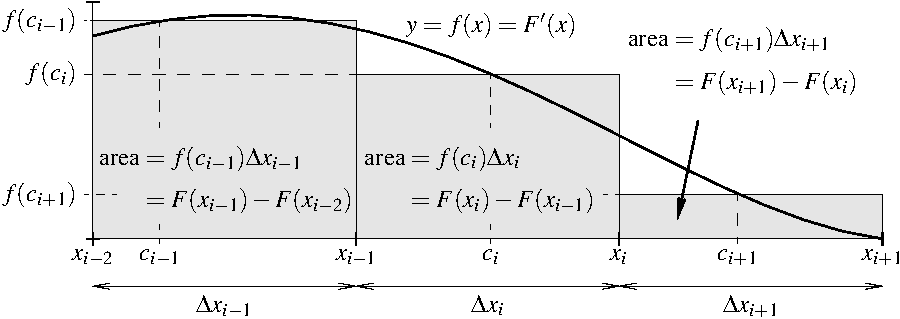
\includegraphics{figures/fundthmfig}
\caption{Mean value theorem on subintervals of a partition
approximating area under the curve.\label{fig:fundthmfig}}
\end{myfigureht}

Using the notation from the definition of the integral, we have
$m_i \leq f(c_i) \leq M_i$ and so
\begin{equation*}
m_i \Delta x_i \leq F(x_i) - F(x_{i-1}) \leq M_i \Delta x_i .
\end{equation*}
We sum over $i = 1,2, \ldots, n$ to get
\begin{equation*}
\sum_{i=1}^n m_i \Delta x_i
\leq \sum_{i=1}^n \bigl(F(x_i) - F(x_{i-1}) \bigr)
\leq \sum_{i=1}^n M_i \Delta x_i .
\end{equation*}
In the middle sum, all the terms except the first and last cancel 
and we end up with $F(x_n)-F(x_0) = F(b)-F(a)$.  The sums on the left
and on the right are the lower and the upper sum respectively.  So
\begin{equation*}
L(P,f) \leq F(b)-F(a) \leq U(P,f) .
\end{equation*}
We take the supremum of $L(P,f)$ over all partitions $P$ and the left inequality
yields 
\begin{equation*}
\underline{\int_a^b} f \leq F(b)-F(a) .
\end{equation*}
Similarly, taking
the infimum of $U(P,f)$ over all partitions $P$ yields
\begin{equation*}
F(b)-F(a) \leq \overline{\int_a^b} f .
\end{equation*}
As $f$ is Riemann integrable, we have
\begin{equation*}
\int_a^b f =
\underline{\int_a^b} f \leq F(b)-F(a) \leq \overline{\int_a^b} f
= \int_a^b f .
\end{equation*}
The inequalities must be equalities and we are done.
\end{proof}

The theorem is used to compute integrals.  Suppose we know that
the function $f(x)$ is a derivative of some other function $F(x)$,
then we can find an explicit expression for $\int_a^b f$. 

\begin{example}
Suppose we are trying to compute
\begin{equation*}
\int_0^1 x^2 ~dx .
\end{equation*}
We notice $x^2$ is the derivative of $\frac{x^3}{3}$.  We
use the fundamental theorem to write 
\begin{equation*}
\int_0^1 x^2 ~dx =
\frac{1^3}{3}
-
\frac{0^3}{3}
= \frac{1}{3}.
\end{equation*}
\end{example}

\subsection{Second form of the theorem}

The second form of the fundamental theorem gives us a way to solve
the differential equation $F'(x) = f(x)$, where $f$ is a known
function and we are trying to find an $F$ that satisfies the equation.

\begin{thm} \label{thm:FTCv2}
Let $f \colon [a,b] \to \R$ be a Riemann integrable function.  Define
\begin{equation*}
F(x) := \int_a^x f .
\end{equation*}
First, $F$ is continuous on $[a,b]$.  Second,
if $f$ is continuous at $c \in [a,b]$, then $F$ is differentiable at $c$
and $F'(c) = f(c)$.
\end{thm}

\begin{proof}
As $f$ is bounded, there is an $M > 0$
such that $\abs{f(x)} \leq M$ for all $x \in [a,b]$.  Suppose $x,y \in [a,b]$
with $x > y$.  Then
\begin{equation*}
\abs{F(x)-F(y)} =
\abs{\int_a^x f - \int_a^y f}
=
\abs{\int_y^x f}
\leq
M\abs{x-y} .
\end{equation*}
By symmetry, the same also holds if $x < y$.
So $F$ is Lipschitz continuous and hence continuous.

Now suppose $f$ is continuous at $c$.
Let $\epsilon > 0$ be given.  Let $\delta > 0$ be such that
for $x \in [a,b]$,
$\abs{x-c} < \delta$ implies $\abs{f(x)-f(c)} < \epsilon$.
In particular,
for such $x$ we have
\begin{equation*}
f(c)-\epsilon < f(x) < f(c) + \epsilon.
\end{equation*}
Thus if $x > c$, then
\begin{equation*}
\bigl(f(c)-\epsilon\bigr) (x-c) \leq \int_c^x f \leq
\bigl(f(c) + \epsilon\bigr)(x-c).
\end{equation*}
When $c > x$, then the inequalities are reversed.  Therefore,
assuming $c \not= x$ we get
\begin{equation*}
f(c)-\epsilon
\leq
\frac{\int_c^{x} f}{x-c}
\leq
f(c)+\epsilon .
\end{equation*}
As 
\begin{equation*}
\frac{F(x)-F(c)}{x-c}
=
\frac{\int_a^{x} f - \int_a^{c} f}{x-c}
=
\frac{\int_c^{x} f}{x-c} ,
\end{equation*}
we have 
\begin{equation*}
\abs{\frac{F(x)-F(c)}{x-c} - f(c)} \leq \epsilon .
\end{equation*}
The result follows.  It is left to the reader to see why is it OK that we
just have a non-strict inequality.
\end{proof}

Of course, if $f$ is continuous on $[a,b]$, then it is automatically Riemann
integrable, $F$ is differentiable on all of $[a,b]$ and $F'(x) = f(x)$ for
all $x \in [a,b]$.

\begin{remark} \label{remark:fundthmbase}
The second form of the fundamental theorem of calculus still holds if
we let $d \in [a,b]$ and define
\begin{equation*}
F(x) := \int_d^x f .
\end{equation*}
That is, we can use any point of $[a,b]$ as our base point.  The proof is
left as an exercise.
\end{remark}

Let us look at what a simple discontinuity can do.  Take $f(x) := -1$ if $x
< 0$, and $f(x) := 1$ if $x \geq 0$.  Let $F(x) := \int_0^x f$.  It is not
difficult to see that $F(x) = \abs{x}$.  Notice that $f$ is discontinuous at
$0$ and $F$ is not differentiable at $0$.  However, the converse in the
theorem does not
hold.
Let $g(x) := 0$ if $x \not= 0$, and $g(0) := 1$.  Letting $G(x) :=
\int_0^x g$, we find that $G(x) = 0$ for all $x$.  So $g$ is discontinuous
at $0$, but $G'(0)$ exists and is equal to 0.

A common misunderstanding of the integral for calculus students is to
think of integrals whose solution cannot be given in closed-form as somehow
deficient.  This is not the case.  Most integrals we write down are not
computable in closed-form.  Even some integrals that we consider
in closed-form are not really such.  For example, how does a computer find
the value of $\ln x$?  One way to do it is to note that
we define the natural log as the antiderivative of $\nicefrac{1}{x}$
such that $\ln 1 = 0$.
Therefore,
\begin{equation*}
\ln x := \int_1^x \nicefrac{1}{s}~ds .
\end{equation*}
Then we can numerically approximate the integral.  Morally,
we did not really ``simplify'' $\int_1^x \nicefrac{1}{s}~ds$ by
writing down $\ln x$.  We simply gave the integral a name.
If we require numerical answers,
it is possible we end up doing
the calculation by approximating an integral anyway.
In the next section, we even define the exponential using
the logarithm, which we define in terms of the integral.

Another common function defined by an integral that cannot
be evaluated symbolically
is the erf function, defined as
\begin{equation*}
\operatorname{erf}(x) := \frac{2}{\sqrt{\pi}} \int_0^x e^{-s^2} ~ds .
\end{equation*}
This function comes up often in applied mathematics.  It is simply 
the antiderivative of $\left(\nicefrac{2}{\sqrt{\pi}}\right) e^{-x^2}$
that is zero at zero.
The second form of the fundamental theorem tells us that we can write the function
as an integral.  If we wish to compute any particular value, we 
numerically approximate the integral.

\subsection{Change of variables}

A theorem often used in calculus to solve integrals is the change of
variables theorem.  Let us prove it now.  Recall 
a function is continuously differentiable if
it is differentiable and the derivative is continuous.

\begin{thm}[Change of variables]
\index{change of variables theorem}
Let $g \colon [a,b] \to \R$ be a continuously differentiable function,
let $f \colon [c,d] \to \R$ be continuous, and suppose
$g([a,b]) \subset [c,d]$.  Then
\begin{equation*}
\int_a^b f\bigl(g(x)\bigr)\, g'(x)~ dx =
\int_{g(a)}^{g(b)} f(s)~ ds .
\end{equation*}
\end{thm}

\begin{proof}
As $g$, $g'$, and $f$ are continuous, we know $f\bigl(g(x)\bigr)\,g'(x)$
is a continuous function on $[a,b]$, therefore it is Riemann integrable.
Similarly, $f$ is integrable on any subinterval of $[c,d]$.

Define 
\begin{equation*}
F(y) := \int_{g(a)}^{y} f(s)~ds .
\end{equation*}
By the second form of the fundamental
theorem of calculus (see \remarkref{remark:fundthmbase} and \exerciseref{secondftc:exercise})
$F$ is a differentiable function and $F'(y) = f(y)$.  We apply the chain
rule and write
\begin{equation*}
\bigl( F \circ g \bigr)' (x) =
F'\bigl(g(x)\bigr) g'(x)
=
f\bigl(g(x)\bigr) g'(x) .
\end{equation*}
We note that $F\bigl(g(a)\bigr) = 0$ and we
use the first form of the fundamental theorem
to obtain
\begin{multline*}
\qquad %to center things more
\int_{g(a)}^{g(b)} f(s)~ds = F\bigl(g(b)\bigr) = F\bigl(g(b)\bigr)-F\bigl(g(a)\bigr)
\\
=
\int_a^b 
\bigl( F \circ g \bigr)' (x) ~dx
=
\int_a^b 
f\bigl(g(x)\bigr) g'(x)
~dx .
\qquad %to center things more
\qedhere
\end{multline*}
\end{proof}

The change of variables theorem is often used to solve integrals by changing them
to integrals that we know or that we can solve using the fundamental theorem of
calculus.

\begin{example}
From an exercise, we know that the derivative of $\sin(x)$ is $\cos(x)$.
Therefore, we solve
\begin{equation*}
\int_0^{\sqrt{\pi}} x \cos(x^2) ~ dx = \int_0^\pi \frac{\cos(s)}{2} ~ ds
=
\frac{1}{2}
\int_0^\pi \cos(s) ~ ds
=
\frac{
\sin(\pi) - \sin(0)
}{2}
=
0 .
\end{equation*}
\end{example}

However, beware that we must satisfy the hypotheses of the theorem.  The
following example demonstrates why we should not just 
move symbols around mindlessly.
We must be careful that those symbols really make sense.

\begin{example}
Suppose we write down
\begin{equation*}
\int_{-1}^{1} \frac{\ln \abs{x}}{x} ~dx .
\end{equation*}
It may be tempting to take $g(x) := \ln \abs{x}$.  Then take $g'(x) =
\frac{1}{x}$ and try to write
\begin{equation*}
\int_{g(-1)}^{g(1)} s ~ds = 
\int_{0}^{0} s ~ds = 0. 
\end{equation*}
This ``solution'' is incorrect, and it does not say
that we can solve the given integral.  First problem is that
$\frac{\ln \abs{x}}{x}$ is not continuous on $[-1,1]$.
It is not defined at 0, and cannot be made continuous by defining a value at
0.
Second, $\frac{\ln \abs{x}}{x}$ is not even Riemann integrable on $[-1,1]$
(it is unbounded).
The integral we wrote down simply does not make sense.
Finally, $g$ is not continuous 
on $[-1,1]$, let alone continuously differentiable.
\end{example}

\subsection{Exercises}

\begin{exercise}
Compute
$\displaystyle
\frac{d}{dx} \biggl( \int_{-x}^x e^{s^2}~ds \biggr)$.
\end{exercise}

\begin{exercise}
Compute
$\displaystyle
\frac{d}{dx} \biggl( \int_{0}^{x^2} \sin(s^2)~ds \biggr)$.
\end{exercise}

\begin{exercise}
Suppose $F \colon [a,b] \to \R$ is continuous and differentiable
on $[a,b] \setminus S$, where $S$ is a finite set.  Suppose there
exists an $f \in \sR[a,b]$ such that $f(x) = F'(x)$ for $x \in [a,b]
\setminus S$.  Show that
$\int_a^b f = F(b)-F(a)$.
\end{exercise}

\begin{exercise} \label{secondftc:exercise}
Let $f \colon [a,b] \to \R$ be a continuous function.  Let $c \in [a,b]$
be arbitrary.  Define
\begin{equation*}
F(x) := \int_c^x f .
\end{equation*}
Prove that $F$ is differentiable and that $F'(x) = f(x)$ for all $x \in
[a,b]$.
\end{exercise}

\begin{exercise}
Prove \emph{\myindex{integration by parts}}.  That is, suppose $F$ and
$G$ are continuously differentiable functions on $[a,b]$.  Then prove
\begin{equation*}
\int_a^b F(x)G'(x)~dx
=
F(b)G(b)-F(a)G(a)
-
\int_a^b F'(x)G(x)~dx .
\end{equation*}
\end{exercise}

\begin{exercise}
Suppose $F$ and $G$ are
continuously\footnote{
Compare this hypothesis to \exerciseref{exercise:samediffconst}.}
differentiable
functions defined on $[a,b]$
such that $F'(x) = G'(x)$ for all $x \in [a,b]$.
Using the fundamental theorem of calculus,
show that $F$ and $G$ differ by a constant.  That is, show that
there exists a $C \in \R$ such that
$F(x)-G(x) = C$.
\end{exercise}

\begin{exnote}
The next exercise shows how we can use the integral to ``smooth out'' a
non-differentiable function.
\end{exnote}

\begin{exercise} \label{exercise:smoothingout}
Let $f \colon [a,b] \to \R$ be a continuous function.  Let $\epsilon > 0$
be a constant.  For $x \in [a+\epsilon,b-\epsilon]$, define
\begin{equation*}
g(x) := \frac{1}{2\epsilon} \int_{x-\epsilon}^{x+\epsilon} f .
\end{equation*}
\begin{enumerate}[a)]
\item
Show that $g$ is differentiable and find the derivative.
\item
Let $f$ be differentiable and fix $x \in (a,b)$ (let $\epsilon$
be small enough).  What happens to $g'(x)$ as $\epsilon$ gets smaller?
\item
Find $g$ for $f(x) := \abs{x}$, $\epsilon = 1$ (you can assume 
$[a,b]$ is large enough).
\end{enumerate}
\end{exercise}

\begin{exercise}
Suppose $f \colon [a,b] \to \R$ is continuous and
$\int_a^x f = \int_x^b f$ for all $x \in [a,b]$.  Show that $f(x) = 0$
for all $x \in [a,b]$.
\end{exercise}

\begin{exercise}
Suppose $f \colon [a,b] \to \R$ is continuous and
$\int_a^x f = 0$ for all rational $x$ in $[a,b]$.  Show that $f(x) = 0$
for all $x \in [a,b]$.
\end{exercise}

\begin{samepage}
\begin{exercise}
A function $f$ is an \emph{\myindex{odd function}} if $f(x) = -f(-x)$,
and $f$ is an \emph{\myindex{even function}} if $f(x) = f(-x)$.  Let $a >
0$.  Assume $f$ is continuous.  Prove:
\begin{enumerate}[a)]
\item
If $f$ is odd, then $\int_{-a}^a f = 0$.
\item
If $f$ is even, then $\int_{-a}^a f = 2 \int_0^a f$.
\end{enumerate}
\end{exercise}
\end{samepage}

\begin{exercise}
{\ }
\begin{enumerate}[a)]
\item
Show that $f(x) := \sin(\nicefrac{1}{x})$
is integrable on any interval (you can define $f(0)$ to be anything).
\item
Compute $\int_{-1}^1 \sin(\nicefrac{1}{x})~dx$.  (Mind the
discontinuity)
\end{enumerate}
\end{exercise}

\begin{exercise}[uses \sectionref{sec:monotonefunc}]
{\ }
\begin{enumerate}[a)]
\item
Suppose $f \colon [a,b] \to \R$ is increasing, by
\propref{prop:monotoneintegrable},
%\exerciseref{exercise:boundedvariationintegrable},
$f$ is Riemann integrable.  Suppose $f$ has a discontinuity at $c \in
(a,b)$, show that $F(x) := \int_a^x f$ is not differentiable at $c$.
\item
In \exerciseref{exercise:increasingfuncdiscatQ}, you constructed an increasing
function $f \colon [0,1] \to \R$ that is discontinuous at every
$x \in [0,1] \cap \Q$.  Use this $f$ to construct a function $F(x)$ that is
continuous on $[0,1]$, but not differentiable at every $x \in [0,1] \cap \Q$.
\end{enumerate}
\end{exercise}

%%%%%%%%%%%%%%%%%%%%%%%%%%%%%%%%%%%%%%%%%%%%%%%%%%%%%%%%%%%%%%%%%%%%%%%%%%%%%%

\sectionnewpage
\section{The logarithm and the exponential}
\label{sec:logandexp}

\sectionnotes{1 lecture (optional, requires the optional sections 
\sectionref{sec:limitatinf},
\sectionref{sec:monotonefunc},
\sectionref{sec:ift})}

We now have all that is required to finally properly define the exponential
and the
logarithm that you know from calculus so well.
First, we have a good idea of what $x^n$ means as long as
$n$ is a positive integer.  Simply,
\begin{equation*}
x^n := \underbrace{x \cdot x \cdot \cdots \cdot x}_{\text{$n$ times}} .
\end{equation*}
It makes sense to define $x^0 := 1$.
For negative integers we define $x^{-n} := \nicefrac{1}{x^n}$.
If $x > 0$,
we defined $x^{1/n}$ as
the unique positive $n$th root.  Finally, for a rational
number $\nicefrac{n}{m}$ (in lowest terms), we define
\begin{equation*}
x^{n/m} := {\bigl(x^{1/m}\bigr)}^n .
\end{equation*}
It is not difficult to show 
we get the same number no matter what
representation of $\nicefrac{n}{m}$ we use, so we do not need to use
lowest terms.

However, what do we mean by $\sqrt{2}^{\sqrt{2}}$?  Or
$x^y$ in general?  In particular, what is $e^x$ for all $x$?
And how do we solve $y=e^x$ for $x$?
This section answers these questions and more.

\subsection{The logarithm}
\index{logarithm}

It is convenient to start with the logarithm.  
Let us show that
a unique function with the right properties exists, and only then will
we call it \emph{the} logarithm.

\begin{prop}
There exists a unique function $L \colon (0,\infty) \to \R$ such that
\begin{enumerate}[(i)]
\item \label{it:log:i}
$L(1) = 0$.
\item \label{it:log:ii}
$L$ is differentiable and $L'(x) = \nicefrac{1}{x}$.
\item \label{it:log:iii}
$L$ is strictly increasing, bijective, and
\begin{equation*}
\lim_{x\to 0} L(x) = -\infty , \qquad \text{and} \qquad
\lim_{x\to \infty} L(x) = \infty .
\end{equation*}
\item \label{it:log:iv}
$L(xy) = L(x)+L(y)$ for all $x,y \in (0,\infty)$.
\item \label{it:log:v}
If $q$ is a rational number and $x > 0$, then
$L(x^q) = q L(x)$.
\end{enumerate}
\end{prop}

\begin{proof}
To prove existence, let us define a candidate and show it satisfies
all the properties.  Define
\begin{equation*}
L(x) := \int_1^x \frac{1}{t}~dt .
\end{equation*}

Obviously \ref{it:log:i} holds.  Property \ref{it:log:ii} holds
via the second form of the fundamental theorem of calculus
(\thmref{thm:FTCv2}).

To prove property \ref{it:log:iv},
we change variables $u=yt$ to obtain
\begin{equation*}
L(x) =
\int_1^{x} \frac{1}{t}~dt
=
\int_y^{xy} \frac{1}{u}~du
=
\int_1^{xy} \frac{1}{u}~du
-
\int_1^{y} \frac{1}{u}~du
=
L(xy)-L(y) .
\end{equation*}

Let us prove \ref{it:log:iii}.
Property \ref{it:log:ii} together with the fact that $L'(x) = \nicefrac{1}{x} > 0$ 
for $x > 0$, implies that $L$
is strictly increasing and hence one-to-one.
Let us show $L$ is onto.  
As $\nicefrac{1}{t} \geq \nicefrac{1}{2}$ when $t \in [1,2]$,
\begin{equation*}
L(2) = \int_1^2 \frac{1}{t} ~dt \geq \nicefrac{1}{2} .
\end{equation*}
By induction, \ref{it:log:iv} implies that for $n \in \N$
\begin{equation*}
L(2^n) = L(2) + L(2) + \cdots + L(2) = n L(2) .
\end{equation*}
Given any $y > 0$, 
by the \hyperref[thm:arch:i]{Archimedean property} of the real numbers
(notice $L(2) > 0$), there is an $n \in \N$ such that
$L(2^n) > y$.  By the
\hyperref[IVT:thm]{intermediate value theorem}
there is an $x_1 \in (1,2^n)$ such that $L(x_1) = y$.  We get
$(0,\infty)$ is in the image of $L$.
As $L$ is increasing, $L(x) > y$ for all $x > 2^n$, and so
\begin{equation*}
\lim_{x\to\infty} L(x) = \infty .
\end{equation*}
Next
$0 = L(\nicefrac{x}{x}) = L(x) + L(\nicefrac{1}{x})$, and
so $L(x) = - L(\nicefrac{1}{x})$.  Using $x=2^{-n}$, we obtain
as above that $L$ achieves all negative numbers.  And
\begin{equation*}
\lim_{x \to 0} L(x) = 
\lim_{x \to 0} -L(\nicefrac{1}{x})
=
\lim_{x \to \infty} -L(x)
=  - \infty .
\end{equation*}
In the limits, note that only $x > 0$ are in the domain of $L$.

Let us now prove \ref{it:log:v}.
As above, \ref{it:log:iv} implies for $n \in \N$ we have
$L(x^n) = n L(x)$.
We already saw that
$L(x) = - L(\nicefrac{1}{x})$
so $L(x^{-n}) = - L(x^n) = -n L(x)$.  Then for $m \in \N$
\begin{equation*}
L(x) = L\Bigl({(x^{1/m})}^m\Bigr) = m L\bigl(x^{1/m}\bigr) .
\end{equation*}
Putting everything together for $n \in \Z$ and $m \in \N$ we have
$L(x^{n/m}) = n L(x^{1/m}) = (\nicefrac{n}{m}) L(x)$.

Finally for uniqueness, let us use properties \ref{it:log:i} and
\ref{it:log:ii}.  Via the first form of the
fundamental theorem of calculus (\thmref{thm:FTCv1}),
\begin{equation*}
L(x) = \int_1^x \frac{1}{t}~dt
\end{equation*}
is the unique function such that $L(1) = 0$ and $L'(x) = \nicefrac{1}{x}$.
\end{proof}

Having proved
that there is a unique function with these properties
we simply define the \emph{\myindex{logarithm}} or sometimes called the
\emph{\myindex{natural logarithm}}:
\glsadd{not:ln}
\begin{equation*}
\ln(x) := L(x) .
\end{equation*}
Often mathematicians write $\log(x)$ instead of $\ln(x)$, which is
more familiar to calculus students.

\subsection{The exponential}
\index{exponential}

Just as with the logarithm we define the exponential via a list of
properties.

\begin{prop}
There exists a unique function $E \colon \R \to (0,\infty)$ such that
\begin{enumerate}[(i)]
\item \label{it:exp:i}
$E(0) = 1$.
\item \label{it:exp:ii}
$E$ is differentiable and $E'(x) = E(x)$.
\item \label{it:exp:iii}
$E$ is strictly increasing, bijective, and
\begin{equation*}
\lim_{x\to -\infty} E(x) = 0 , \qquad \text{and} \qquad
\lim_{x\to \infty} E(x) = \infty .
\end{equation*}
\item \label{it:exp:iv}
$E(x+y) = E(x)E(y)$ for all $x,y \in \R$.
\item \label{it:exp:v}
If $q \in \Q$, then
$E(qx) = {E(x)}^q$.
\end{enumerate}
\end{prop}

\begin{proof}
Again, we prove existence of such a function by defining a candidate,
and prove that it satisfies all the properties.
The $L$ defined above is invertible.  Let $E$ be the
inverse function of $L$.  Property \ref{it:exp:i} is immediate.

Property \ref{it:exp:ii} follows
via the inverse function theorem, in particular
\lemmaref{lemma:ift}:  $L$ satisfies
all the hypotheses of the lemma, and hence
\begin{equation*}
E'(x) = \frac{1}{L'\bigl(E(x)\bigr)} = E(x) .
\end{equation*}

Let us look at property \ref{it:exp:iii}.
The function $E$ is strictly increasing since 
$E'(x) = E(x) > 0$.  As $E$ is the inverse of $L$, it must also
be bijective.  
To find the limits, we use that 
$E$ is strictly increasing and onto $(0,\infty)$.
For every $M > 0$, there is an $x_0$ such that
$E(x_0) = M$ and $E(x) \geq M$ for all $x \geq x_0$.
Similarly, for every $\epsilon > 0$, there is
an $x_0$ such that $E(x_0) = \epsilon$ and
$E(x) < \epsilon$ for all $x < x_0$.
Therefore,
\begin{equation*}
\lim_{n\to -\infty} E(x) = 0 , \qquad \text{and} \qquad
\lim_{n\to \infty} E(x) = \infty .
\end{equation*}

To prove property \ref{it:exp:iv} we use the corresponding
property for the logarithm.
Take $x, y \in \R$.
As $L$ is bijective, find $a$ and $b$ such that $x = L(a)$ and $y = L(b)$.  Then
\begin{equation*}
E(x+y) =
E\bigl(L(a)+L(b)\bigr) = 
E\bigl(L(ab)\bigr) = ab = E(x)E(y)  .
\end{equation*}

Property \ref{it:exp:v} also follows from the corresponding property of $L$.
Given $x \in \R$, let $a$ be such that $x = L(a)$ and
\begin{equation*}
E(qx) = E\bigl(qL(a)\bigr)
E\bigl(L(a^q)\bigr) = a^q = {E(x)}^q .
\end{equation*}

Finally, uniqueness follows from
\ref{it:exp:i} and
\ref{it:exp:ii}.
Let $E$ and $F$
be two functions satisfying
\ref{it:exp:i} and \ref{it:exp:ii}.  
\begin{equation*}
\frac{d}{dx} \Bigl( F(x)E(-x) \Bigr)
=
F'(x)E(-x) - E'(-x)F(x)
=
F(x)E(-x) - E(-x)F(x) = 0 .
\end{equation*}
Therefore, by \propref{prop:derzeroconst},
$F(x)E(-x) = F(0)E(-0) = 1$ for all $x \in \R$.
Next, $1 = E(0) = E(x-x) = E(x)E(-x)$.
%Doing the computation with $F = E$,
%we obtain $E(x)E(-x) = 1$.
Then
\begin{equation*}
0 = 1-1 = F(x)E(-x) - E(x)E(-x) = \bigl(F(x)-E(x)\bigr) E(-x) .
\end{equation*}
%Since $E(x)E(-x) = 1$,
Finally, $E(-x) \not= 0$\footnote{%
$E$ is a function into $(0,\infty)$ after all.
However, $E(-x) \neq 0$ also follows
from $E(x)E(-x) = 1$.  Therefore, we can prove uniqueness of $E$ 
given \ref{it:exp:i} and \ref{it:exp:ii}, even for functions $E \colon \R
\to \R$.}
for all $x \in \R$.
So
$F(x)-E(x) = 0$ for all $x$, and we are done.
\end{proof}

Having proved $E$ is unique, we define the
\emph{\myindex{exponential}} function as
\glsadd{not:exp}
\begin{equation*}
\exp(x) := E(x) .
\end{equation*}

If $y \in \Q$ and $x > 0$, then
\begin{equation*}
x^y = \exp\bigl(\ln(x^y)\bigr) = \exp\bigl(y\ln(x)\bigr) .
\end{equation*}
We can now make sense of exponentiation $x^y$ for arbitrary $y \in \R$;
if $x > 0$ and $y$ is irrational, define
\glsadd{not:pow}
\begin{equation*}
x^y := \exp\bigl(y\ln(x)\bigr) .
\end{equation*}
As $\exp$ is continuous then $x^y$ is a continuous function of $y$.
Therefore, we would
obtain the same result had we taken a sequence of rational numbers $\{ y_n \}$
approaching $y$ and defined $x^y = \lim\, x^{y_n}$.

Define the number $e$,
sometimes called \emph{\myindex{Euler's number}} or
the \emph{\myindex{base of the natural logarithm}}, as
\glsadd{not:e}
\begin{equation*}
e := \exp(1) .
\end{equation*}
Let us justify the notation $e^x$ for $\exp(x)$:
\begin{equation*}
e^x = \exp\bigl(x \ln(e) \bigr) = \exp(x) .
\end{equation*}

Let us extend properties of logarithm and exponential to
irrational powers.  The proof is immediate.

\begin{prop}
Let $x, y \in \R$.
\begin{enumerate}[(i)]
\item
$\exp(xy) = {\bigl(\exp(x)\bigr)}^y$.
\item
If $x > 0$ then $\ln(x^y) = y \ln (x)$.
\end{enumerate}
\end{prop}

\begin{remark}
There are other equivalent ways to define the exponential and the logarithm.
A common way is to define $E$ as the solution to the differential equation
$E'(x) = E(x)$, $E(0) = 1$.  See \exampleref{example:picardexponential},
for a sketch of that approach.  Yet another
approach is to define the exponential function by
power series, see \exampleref{example:exponentialbypowerseries}.
\end{remark}

\begin{remark}
We have proved the uniqueness of the functions $L$ and $E$ from
just the properties $L(1)=0$, $L'(x) = \nicefrac{1}{x}$
and the equivalent condition for the exponential
$E'(x) = E(x)$, $E(0) = 1$.  Existence in fact also follows
from just these properties.
Alternatively, uniqueness also follows
from the laws of exponents, see the exercises.
\end{remark}

\subsection{Exercises}

\begin{exercise}
Let $y$ be any real number and $b > 0$.  Define $f \colon (0,\infty) \to \R$
and $g \colon \R \to \R$ as, $f(x) := x^y$ and $g(x) := b^x$.  Show that $f$
and $g$ are differentiable and find their derivative.
\end{exercise}

\begin{samepage}
\begin{exercise}
Let $b > 0$, $b\neq 1$ be given.
\begin{enumerate}[a)]
\item
Show that for every $y > 0$, there exists a unique number $x$
such that $y = b^x$.  Define
the \emph{\myindex{logarithm base $b$}},
$\log_b \colon (0,\infty) \to \R$, by
$\log_b(y) := x$.
\item
Show that $\log_b(x) = \frac{\ln(x)}{\ln(b)}$.
\item
Prove that if $c > 0$, $c \neq 1$, then
$\log_b(x) = \frac{\log_c(x)}{\log_c(b)}$.
\item
Prove $\log_b(xy) =
\log_b(x)+\log_b(y)$, and $\log_b(x^y) = y \log_b(x)$.
\end{enumerate}
\end{exercise}
\end{samepage}

\begin{exercise}[requires \sectionref{sec:taylor}]
Use \hyperref[thm:taylor]{Taylor's theorem} to study the remainder term and show that for
all $x \in \R$
\begin{equation*}
e^x = \sum_{n=0}^\infty \frac{x^n}{n!} .
\end{equation*}
Hint: Do not differentiate the series term by term (unless you would prove that it
works).
\end{exercise}

\begin{exercise}
Use the geometric sum formula to show (for $t\not= -1$)
\begin{equation*}
1-t+t^2-\cdots+{(-1)}^n t^n = \frac{1}{1+t} - \frac{{(-1)}^{n+1}t^{n+1}}{1+t}.
\end{equation*}
Using this fact show
\begin{equation*}
\ln (1+x) = \sum_{n=1}^\infty \frac{{(-1)}^{n+1}x^n}{n} 
\end{equation*}
for all $x \in (-1,1]$ (note that $x=1$ is included).  Finally,
find the limit of the alternating harmonic series
\begin{equation*}
\sum_{n=1}^\infty \frac{{(-1)}^{n+1}}{n} = 1 - \nicefrac{1}{2} +
\nicefrac{1}{3} - \nicefrac{1}{4} + \cdots
\end{equation*}
\end{exercise}

\begin{exercise}
Show 
\begin{equation*}
e^x = \lim_{n\to\infty} {\left( 1 + \frac{x}{n} \right)}^n .
\end{equation*}
Hint: Take the logarithm.\\
Note: The expression 
${\left( 1 + \frac{x}{n} \right)}^n$ arises in compound interest
calculations.  It is the amount of money in a bank account after 1 year
if 1 dollar was deposited initially at interest $x$
and the interest was compounded $n$
times during the year.  The exponential $e^x$ is the result of continuous
compounding.
\end{exercise}

\begin{samepage}
\begin{exercise}
{\ }
\begin{enumerate}[a)]
\item
Prove that for $n \in \N$ we have
\begin{equation*}
\sum_{k=2}^{n}
\frac{1}{k}
\leq
\ln (n)
\leq
\sum_{k=1}^{n-1}
\frac{1}{k} .
\end{equation*}
\item
Prove that the limit
\begin{equation*}
\gamma := \lim_{n\to\infty}
\left( \sum_{k=1}^{n}
\frac{1}{k} - \ln (n) \right)
\end{equation*}
exists.  This constant is known as the
\emph{\myindex{Euler--Mascheroni constant}}%
\footnote{Named for the Swiss mathematician
\href{https://en.wikipedia.org/wiki/Leonhard_Euler}{Leonhard Paul Euler}
(1707--1783)
and the Italian mathematician
\href{https://en.wikipedia.org/wiki/Lorenzo_Mascheroni}{Lorenzo Mascheroni}
(1750--1800).}.  It is not known if this constant is rational or not.
It is approximately $\gamma \approx 0.5772$.
\end{enumerate}
\end{exercise}
\end{samepage}

\begin{exercise}
Show
\begin{equation*}
\lim_{x\to\infty} \frac{\ln(x)}{x} = 0 .
\end{equation*}
\end{exercise}

\begin{exercise}
Show that $e^x$ is \emph{\myindex{convex}}, in other words, show that 
if $a \leq x \leq b$ then
$e^x \leq e^a \frac{b-x}{b-a} + e^b \frac{x-a}{b-a}$.
\end{exercise}

\begin{exercise}
Using the logarithm find
\begin{equation*}
%\lim_{n\to\infty} {\left( 1 + \nicefrac{1}{n} \right)}^n = e .
\lim_{n\to\infty} n^{1/n} .
\end{equation*}
\end{exercise}

\begin{exercise}
Show that $E(x) = e^x$ is the unique continuous function such that
$E(x+y) = E(x)E(y)$ and $E(1) = e$.   Similarly, prove that $L(x) = \ln(x)$
is the unique continuous
function defined on positive $x$ such that $L(xy) = L(x)+L(y)$
and $L(e) = 1$.
\end{exercise}

\begin{exercise}[requires \sectionref{sec:taylor}]\label{exercise:nonanalytic}
Since $(e^x)' = e^x$, it is easy to see that $e^x$ is
\myindex{infinitely differentiable}\index{differentiable!infinitely}
(has derivatives of all orders).  Define the function $f \colon \R \to \R$.
\begin{equation*}
f(x) := \begin{cases}
e^{-1/x} & \text{if $x > 0$,} \\
0 & \text{if $x \leq 0$}.
\end{cases}
\end{equation*}
\begin{enumerate}[a)]
\item
Prove that for any $m \in \N$,
\begin{equation*}
\lim_{x \to 0^+} \frac{e^{-1/x}}{x^m} = 0 .
\end{equation*}
\item
Prove that $f$ is infinitely differentiable.
\item
Compute the Taylor series for $f$ at the origin, that is,
\begin{equation*}
\sum_{k=0}^\infty
\frac{f^{(k)}(0)}{k!}x^k .
\end{equation*}
Show that it converges, but show that it does not converge to $f(x)$
for any $x > 0$.
\end{enumerate}
\end{exercise}

%%%%%%%%%%%%%%%%%%%%%%%%%%%%%%%%%%%%%%%%%%%%%%%%%%%%%%%%%%%%%%%%%%%%%%%%%%%%%%

\sectionnewpage
\section{Improper integrals}
\label{sec:impropriemann}

\sectionnotes{2--3 lectures (optional section, can safely be skipped, 
requires the optional \sectionref{sec:limitatinf})}

Often it is necessary to integrate over the
entire real line, or a unbounded interval of the form $[a,\infty)$ or
$(-\infty,b]$.  Also, we may wish to integrate unbounded functions
defined on a open bounded interval $(a,b)$.
Such functions are not Riemann integrable, but we may want to write down
the integral anyway in the spirit of \lemmaref{lemma:boundedimpriemann}.
These integrals are called \emph{\myindex{improper integrals}},
and are limits
of integrals rather than integrals themselves.

\begin{defn}
Suppose $f \colon [a,b) \to \R$ is a function (not necessarily bounded)
that is Riemann integrable on $[a,c]$ for all $c < b$.  We define
\begin{equation*}
\int_a^b f := \lim_{c \to b^-} \int_a^{c} f ,
\end{equation*}
if the limit exists.

Suppose $f \colon [a,\infty) \to \R$ is a function such that
$f$ is Riemann integrable on $[a,c]$ for all $c < \infty$.  
We define
\begin{equation*}
\int_a^\infty f := \lim_{c \to \infty} \int_a^c f ,
\end{equation*}
if the limit exists.

If the limit exists, we say the improper integral
\emph{converges}\index{convergent!improper integral}.
If the limit does not exist, we say the improper integral
\emph{diverges}\index{divergent!improper integral}.

We similarly define improper integrals for the left-hand endpoint, we leave
this to the reader.
\end{defn}

For a finite endpoint $b$,
using \lemmaref{lemma:boundedimpriemann} we see that if
$f$ is bounded, then we defined nothing new.  What is new is that
we can apply this definition to unbounded functions.
The following set of examples is
so useful that we state it as a proposition.

\begin{prop}[$p$-test for integrals]%
\index{p-test for integrals@$p$-test for integrals}
\label{impropriemann:ptest}
The improper integral
\begin{equation*}
\int_1^\infty \frac{1}{x^p} ~dx
\end{equation*}
converges to $\frac{1}{p-1}$ if $p > 1$ and diverges if $0 < p \leq 1$.

The improper integral
\begin{equation*}
\int_0^1 \frac{1}{x^p} ~dx
\end{equation*}
converges to $\frac{1}{1-p}$ if $0 < p < 1$ and diverges if $p \geq 1$.
\end{prop}

\begin{proof}
The proof follows by application of the fundamental theorem of calculus.
Let us do the proof for $p > 1$ for the infinite right endpoint and
leave the rest to the reader.  Hint: You should handle $p=1$
separately.

Suppose $p > 1$.  Then
\begin{equation*}
\int_1^b \frac{1}{x^p} ~dx
=
\int_1^b x^{-p} ~dx
=
\frac{b^{-p+1}}{-p+1}
-
\frac{1^{-p+1}}{-p+1}
=
\frac{-1}{(p-1)b^{p-1}}
+
\frac{1}{p-1} .
\end{equation*}
As $p > 1$, then $p-1 > 0$.  Take the limit as $b \to \infty$
to obtain that $\frac{1}{b^{p-1}}$ goes to 0.  The result follows.
\end{proof}

We state the following proposition for just one type
of improper integral, though the proof is straight
forward and the same for other types of improper integrals.

\begin{prop} \label{impropriemann:tail}
Let $f \colon [a,\infty) \to \R$ be a function
that is Riemann integrable on $[a,b]$ for all $b > a$.
Given any $b > a$,
$\int_b^\infty f$ converges if and only if $\int_a^\infty f$
converges, in which case
\begin{equation*}
\int_a^\infty f
=
\int_a^b f +
\int_b^\infty f .
\end{equation*}
\end{prop}

\begin{proof}
Let $c > b$.  Then
\begin{equation*}
\int_a^c f
=
\int_a^b f +
\int_b^c f .
\end{equation*}
Taking the limit $c \to \infty$ finishes the proof.
\end{proof}

Nonnegative functions are easier to work with
as the following proposition demonstrates.
The exercises will show that this proposition
holds only for nonnegative functions.
Analogues of this proposition
exist for all the other types of improper limits are left to the
student.

\begin{prop} \label{impropriemann:possimp}
Suppose $f \colon [a,\infty) \to \R$ is nonnegative ($f(x)
\geq 0$ for all $x$) and such that
$f$ is Riemann integrable on $[a,b]$ for all $b > a$.
\begin{enumerate}[(i)]
\item 
\begin{equation*}
\int_a^\infty f = \sup \left\{ \int_a^x f : x \geq a \right\} .
\end{equation*}
\item
Suppose $\{ x_n \}$
is a sequence with $\lim\, x_n = \infty$.  Then
$\int_a^\infty f$ converges if and only if $\lim\, \int_a^{x_n} f$ exists, in
which case
\begin{equation*}
\int_a^\infty f = \lim_{n\to\infty} \int_a^{x_n} f .
\end{equation*}
\end{enumerate}
\end{prop}

In the first item we allow for the value of $\infty$ in the
supremum indicating that the integral diverges to infinity.

\begin{proof}
Let us start with the first item.
Notice that as $f$ is nonnegative,
then $\int_a^x f$ is increasing as a function of $x$.
If the supremum is infinite, then for every $M \in \R$
we find $N$ such that $\int_a^N f \geq M$.  As $\int_a^x f$
is increasing then $\int_a^x f \geq M$ for all $x \geq N$.  So
$\int_a^\infty f$ diverges to infinity.

Next suppose the supremum is finite, say
$A = \sup \left\{ \int_a^x f : x \geq a \right\}$.
For every $\epsilon > 0$, we find an $N$ such that
$A - \int_a^N f < \epsilon$.  As $\int_a^x f$ is increasing,
then
$A - \int_a^x f < \epsilon$ for all $x \geq N$ and hence
$\int_a^\infty f$ converges to $A$.

Let us look at the second item.
If $\int_a^\infty f$ converges then every sequence $\{ x_n \}$ going to
infinity works.  The trick is
proving the other direction.  Suppose $\{ x_n \}$ is such that $\lim\, x_n =
\infty$ and
\begin{equation*}
\lim_{n\to\infty} \int_a^{x_n} f = A
\end{equation*}
converges.  Given $\epsilon > 0$, pick $N$ such that for
all $n \geq N$ we have
$A - \epsilon < \int_a^{x_n} f < A + \epsilon$.
Because $\int_a^x f$ is increasing as a function of $x$, we have that for all
$x \geq x_N$
\begin{equation*}
A - \epsilon < \int_a^{x_N} \leq \int_a^x f .
\end{equation*}
As $\{ x_n \}$ goes to $\infty$, then for any given
$x$, there is an $x_m$ such that $m \geq N$ and $x \leq x_m$.  Then
\begin{equation*}
\int_a^{x} f \leq \int_a^{x_m} f < A + \epsilon .
\end{equation*}
In particular, for all $x \geq x_N$ we have
$\abs{\int_a^{x} f - A} < \epsilon$.
\end{proof}

\begin{prop}[\myindex{Comparison test for improper integrals}]
Let
$f \colon [a,\infty) \to \R$ and
$g \colon [a,\infty) \to \R$ be functions
that are Riemann integrable on $[a,b]$ for all $b > a$.   Suppose
that for all $x \geq a$ we have
\begin{equation*}
\abs{f(x)} \leq g(x) .
\end{equation*}
\begin{enumerate}[(i)]
\item If $\int_a^\infty g$ converges, then $\int_a^\infty f$ converges,
and in this case 
$\abs{\int_a^\infty f} \leq \int_a^\infty g$.
\item If $\int_a^\infty f$ diverges, then $\int_a^\infty g$ diverges.
\end{enumerate}
\end{prop}

\begin{proof}
Let us start with the first item.
For any $b$ and $c$, such that $a \leq b \leq c$, we have 
$-g(x) \leq f(x) \leq g(x)$, and so
\begin{equation*}
\int_b^c -g \leq \int_b^c f \leq \int_b^c g  .
\end{equation*}
In other words, $\abs{\int_b^c f} \leq \int_b^c g$.

Let $\epsilon > 0$ be given.  Because
of \propref{impropriemann:tail} we have
\begin{equation*}
\int_a^\infty g =
\int_a^b g +
\int_b^\infty g .
\end{equation*}
As $\int_a^b g$ goes to
$\int_a^\infty g$ as $b$ goes to infinity, then
$\int_b^\infty g$ goes to 0 as $b$ goes to infinity.  Choose $B$
such that
\begin{equation*}
\int_B^\infty g < \epsilon .
\end{equation*}
As $g$ is nonnegative, then if $B \leq b < c$, then
$\int_b^c g < \epsilon$ as well.
Let $\{ x_n \}$ be a sequence going to infinity.  Let $M$ be such that
$x_n \geq B$ for all $n \geq M$.  Take $n, m \geq M$,
with $x_n \leq x_m$,
\begin{equation*}
\abs{\int_a^{x_m} f - \int_a^{x_n} f} 
=
\abs{\int_{x_n}^{x_m} f} 
\leq \int_{x_n}^{x_m} g < \epsilon .
\end{equation*}
Therefore, the sequence $\{ \int_a^{x_n} f \}_{n=1}^\infty$ is Cauchy and hence converges.

We need to show that the limit is unique.  Suppose $\{ x_n \}$ is a sequence
converging to infinity such that
$\{ \int_a^{x_n} f \}$ converges to $L_1$, and $\{ y_n \}$ is a sequence
converging to infinity is such that
$\{ \int_a^{y_n} f \}$ converges to $L_2$.  Then there must be some $n$ such
that
$\abs{\int_a^{x_n} f - L_1} < \epsilon$ and 
$\abs{\int_a^{y_n} f - L_2} < \epsilon$.  We can also suppose $x_n \geq B$
and $y_n \geq B$.  Then
\begin{equation*}
\abs{L_1 - L_2} \leq
\abs{L_1 - \int_a^{x_n} f}
+
\abs{\int_a^{x_n} f- \int_a^{y_n} f}
+
\abs{\int_a^{y_n} f - L_2}
<
\epsilon
+
\abs{\int_{x_n}^{y_n} f}
+
\epsilon
<
3 \epsilon.
\end{equation*}
As $\epsilon > 0$ was arbitrary, $L_1 = L_2$, and hence
$\int_a^\infty f$ converges.
Above we have shown that $\abs{\int_a^c f} \leq \int_a^c g$ for all $c > a$.
By taking the limit $c \to \infty$, the first item is proved.

The second item is simply a contrapositive of the first item.
\end{proof}

\begin{example}
The improper integral
\begin{equation*}
\int_0^\infty \frac{\sin(x^2)(x+2)}{x^3+1} ~dx
\end{equation*}
converges.

Proof:  First observe we simply need to show
that the integral converges when going from 1 to infinity.
For $x \geq 1$ we obtain
\begin{equation*}
\abs{\frac{\sin(x^2)(x+2)}{x^3+1}}
\leq
\frac{x+2}{x^3+1}
\leq \frac{x+2}{x^3} \leq
\frac{x+2x}{x^3} \leq \frac{3}{x^2} .
\end{equation*}
Then
\begin{equation*}
3 \int_1^\infty \frac{1}{x^2}~dx
=
\lim_{c\to\infty} \int_1^c \frac{3}{x^2} ~dx.
\end{equation*}
So the integral converges.
\end{example}

\begin{example}
You should be careful when doing formal manipulations with improper
integrals.
For example,
\begin{equation*}
\int_2^\infty \frac{2}{x^2-1}~dx
\end{equation*}
converges via the comparison test again using $\frac{1}{x^2}$.  However, if you
succumb to the temptation to write
\begin{equation*}
\frac{2}{x^2-1} = 
\frac{1}{x-1}
-
\frac{1}{x+1} 
\end{equation*}
and try to integrate each part separately, you will not succeed.
It is \emph{not} true that you can split the improper
integral in two; you cannot split the limit.
\begin{equation*}
\begin{split}
\int_2^\infty \frac{2}{x^2-1} ~dx &=
\lim_{b\to \infty} \int_2^b \frac{2}{x^2-1} ~dx
\\
&=
\lim_{b\to \infty}
\left(
\int_2^b \frac{1}{x-1}~dx
-
\int_2^b \frac{1}{x+1}~dx
\right)
\\
&\not=
\int_2^\infty \frac{1}{x-1}~dx
-
\int_2^\infty \frac{1}{x+1}~dx .
\end{split}
\end{equation*}
The last line in the computation does not even make sense.  Both of the
integrals there diverge to infinity since we can
apply the comparison test appropriately with
$\nicefrac{1}{x}$.  We get $\infty - \infty$.
\end{example}

Now let us suppose that we need to take limits at both endpoints.

\begin{defn}
Suppose $f \colon (a,b) \to \R$ is a function
that is Riemann integrable on $[c,d]$ for all $c$, $d$
such that $a < c < d < b$, then we define
\begin{equation*}
\int_a^b f := \lim_{c \to a^+} \, \lim_{d \to b^-} \, \int_{c}^{d} f ,
\end{equation*}
if the limits exist.

Suppose $f \colon \R \to \R$ is a function such that
$f$ is Riemann integrable on all bounded intervals $[a,b]$.  Then
we define
\begin{equation*}
\int_{-\infty}^\infty f := \lim_{c \to -\infty} \, \lim_{d \to \infty} \, \int_c^d f ,
\end{equation*}
if the limits exist.

We similarly define improper integrals with one infinite and one finite
improper endpoint, we leave this to the reader.
\end{defn}

One ought to always be careful about double limits.  The definition
given above says that we first take the limit as $d$ goes to $b$ or
$\infty$ for a fixed $c$, and then we take the limit in $c$.
We will have to prove that in this case it does not matter which limit
we compute first.

\begin{example}
Let us see an example:
\begin{equation*}
\int_{-\infty}^\infty \frac{1}{1+x^2} ~ dx
=
\lim_{a \to -\infty} \, \lim_{b \to \infty} \,
\int_{a}^b \frac{1}{1+x^2} ~ dx
=
\lim_{a \to -\infty} \, \lim_{b \to \infty}
\bigl( \arctan(b) - \arctan(a) \bigr)
=
\pi .
\end{equation*}
\end{example}

In the definition the order of the limits can always be switched if they
exist.  Let us prove this fact only for the infinite limits.

\begin{prop}
If $f \colon \R \to \R$ is a function integrable on every bounded interval
$[a,b]$.
Then 
\begin{equation*}
\lim_{a \to -\infty} \, \lim_{b \to \infty} \, \int_a^b f
\quad \text{converges if and only if} \qquad
\lim_{b \to \infty}
\,
\lim_{a \to -\infty}
\,
\int_a^b f
\quad
\text{converges,}
\end{equation*}
in which case the two
expressions are equal.  If either of the
expressions converges then the improper integral converges and
\begin{equation*}
\lim_{a\to\infty}
\int_{-a}^a f
=
\int_{-\infty}^\infty f .
\end{equation*}
\end{prop}

\begin{proof}
Without loss of generality assume $a < 0$ and $b > 0$.  Suppose
the first expression converges.  Then
\begin{equation*}
\begin{split}
\lim_{a \to -\infty} \, \lim_{b \to \infty} \, \int_a^b f
& =
\lim_{a \to -\infty} \, \lim_{b \to \infty}
\left(
\int_a^0 f
+
\int_0^b f
\right)
=
\left(
\lim_{a \to -\infty}
\int_a^0 f
\right)
+
\left(
 \lim_{b \to \infty}
\int_0^b f
\right) \\
& = 
 \lim_{b \to \infty}
\left(
\left(
\lim_{a \to -\infty}
\int_a^0 f
\right) 
+
\int_0^b f
\right)
=
 \lim_{b \to \infty} \,
\lim_{a \to -\infty}
\left(
\int_a^0 f
+
\int_0^b f
\right)  .
\end{split}
\end{equation*}
Similar computation shows the other direction.  Therefore, if
either expression converges then the improper integral converges
and
\begin{equation*}
\begin{split}
\int_{-\infty}^\infty f
=
\lim_{a \to -\infty} \, \lim_{b \to \infty} \, \int_a^b f
& =
\left(
\lim_{a \to -\infty}
\int_a^0 f
\right)
+
\left(
 \lim_{b \to \infty}
\int_0^b f
\right)
\\
& =
\left(
\lim_{a \to \infty}
\int_{-a}^0 f
\right)
+
\left(
 \lim_{a \to \infty}
\int_0^a f
\right)
=
\lim_{a \to \infty}
\left(
\int_{-a}^0 f
+
\int_0^a f
\right)
=
\lim_{a \to \infty}
\int_{-a}^a f .
\end{split}
\end{equation*}
\end{proof}

\begin{example}
On the other hand, you must be careful to
take the limits independently before you know convergence.  Let
$f(x) = \frac{x}{\abs{x}}$ for $x \not= 0$ and $f(0) = 0$.
If $a < 0$ and $b > 0$, then
\begin{equation*}
\int_{a}^b f
=
\int_{a}^0 f
+
\int_{0}^b f
=
a+b .
\end{equation*}
For any fixed $a < 0$ the limit as $b \to \infty$ is infinite, so even
the first limit does not exist, and hence the improper integral
$\int_{-\infty}^\infty f$
does not converge.  On the other hand if $a > 0$, then
\begin{equation*}
\int_{-a}^{a} f
=
(-a)+a = 0 .
\end{equation*}
Therefore,
\begin{equation*}
\lim_{a\to\infty}
\int_{-a}^{a} f
= 0 .
\end{equation*}
\end{example}

\begin{example}
An example to keep in mind for improper integrals
is the so-called \emph{\myindex{sinc function}}%
\footnote{Shortened from Latin: \emph{sinus cardinalis}}.
This function comes up quite often
in both pure and applied mathematics.  Define
\begin{equation*}
\operatorname{sinc}(x) =
\begin{cases}
\frac{\sin(x)}{x} & \text{if $x \not= 0$} , \\
1 & \text{if $x = 0$} .
\end{cases}
\end{equation*}
\begin{myfigureht}
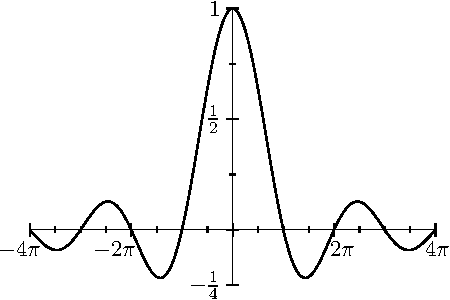
\includegraphics{figures/sincfig}
\caption{The sinc function.
\label{figsinc}}
\end{myfigureht}

It is not difficult to show that
the sinc function is continuous at zero, but that is
not important right now.  What is important is that
\begin{equation*}
\int_{-\infty}^\infty \operatorname{sinc}(x) ~dx = \pi ,
\qquad \text{while} \qquad
\int_{-\infty}^\infty \abs{\operatorname{sinc}(x)} ~dx = \infty .
\end{equation*}
The integral of the sinc function is a continuous analogue of the
alternating harmonic series $\sum \nicefrac{{(-1)}^n}{n}$, while the
absolute value is like the regular harmonic series $\sum \nicefrac{1}{n}$.
In particular, the fact that the integral converges must be done directly
rather than using comparison test.

We will not prove the first statement exactly.  Let us simply prove
that the integral of the sinc function converges, but we will not worry
about the exact limit.  Because $\frac{\sin(-x)}{-x} = \frac{\sin(x)}{x}$, it is
enough to show that
\begin{equation*}
\int_{2\pi}^\infty \frac{\sin(x)}{x}~dx
\end{equation*}
converges.  We
also avoid $x=0$ this way to make our life simpler.

For any $n \in \N$, we have that for $x \in [\pi 2n, \pi (2n+1)]$
\begin{equation*}
\frac{\sin(x)}{\pi (2n+1)}
\leq
\frac{\sin(x)}{x}
\leq
\frac{\sin(x)}{\pi 2n} ,
\end{equation*}
as $\sin(x) \geq 0$.  On $x \in [\pi (2n+1), \pi (2n+2)]$
\begin{equation*}
\frac{\sin(x)}{\pi (2n+1)}
\leq
\frac{\sin(x)}{x}
\leq
\frac{\sin(x)}{\pi (2n+2)} ,
\end{equation*}
as $\sin(x) \leq 0$.

Via the fundamental theorem of calculus,
\begin{equation*}
\frac{2}{\pi (2n+1)}
=
\int_{\pi 2n}^{\pi (2n+1)}
\frac{\sin(x)}{\pi (2n+1)}
~dx
\leq
\int_{\pi 2n}^{\pi (2n+1)}
\frac{\sin(x)}{x}
~dx
\leq
\int_{\pi 2n}^{\pi (2n+1)}
\frac{\sin(x)}{\pi 2n}
~dx
=
\frac{1}{\pi n} .
\end{equation*}
Similarly,
\begin{equation*}
\frac{-2}{\pi (2n+1)}
\leq
\int_{\pi (2n+1)}^{\pi (2n+2)}
\frac{\sin(x)}{x}
~dx
\leq
\frac{-1}{\pi (n+1)} .
\end{equation*}
Adding the two together we find
\begin{equation*}
0
=
\frac{2}{\pi (2n+1)}
+
\frac{-2}{\pi (2n+1)}
\leq
\int_{2\pi n}^{2\pi (n+1)}
\frac{\sin(x)}{x}
~dx
\leq
\frac{1}{\pi n} 
+
\frac{-1}{\pi (n+1)} 
=
\frac{1}{\pi n(n+1)} .
\end{equation*}
See \figureref{fig:sincbound}.
\begin{myfigureht}
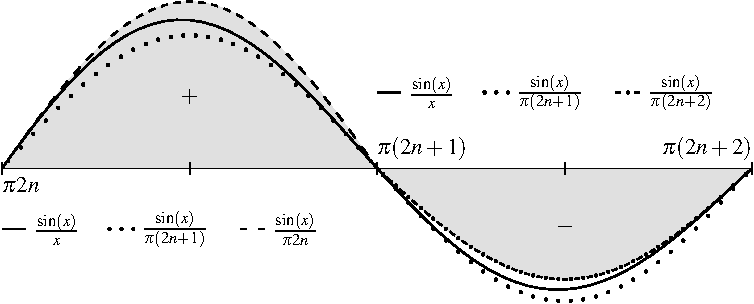
\includegraphics{figures/sincbound}
\caption{Bound of $\int_{2\pi n}^{2\pi (n+1)} \frac{\sin(x)}{x} ~dx$ using
the shaded integral (signed area
$\frac{1}{\pi n} 
+
\frac{-1}{\pi (n+1)}$).\label{fig:sincbound}}
\end{myfigureht}

For $k \in \N$, 
\begin{equation*}
\int_{2\pi}^{2k\pi} \frac{\sin(x)}{x} ~dx
=
\sum_{n=1}^{k-1}
\int_{2\pi n}^{2\pi (n+1)} \frac{\sin(x)}{x} ~dx 
\leq
\sum_{n=1}^{k-1}
\frac{1}{\pi n(n+1)} .
\end{equation*}
We find the partial sums of a series with positive terms.
The series
converges as
$\sum \frac{1}{\pi n (n+1)}$ is a convergent series.  Thus
as a sequence,
\begin{equation*}
\lim_{k\to \infty} \int_{2\pi}^{2k\pi} \frac{\sin(x)}{x} ~dx
=L \leq
\sum_{n=1}^{\infty}
\frac{1}{\pi n(n+1)} < \infty .
\end{equation*}

Let $M > 2\pi$ be arbitrary, and let $k \in \N$
be the largest integer such that $2k\pi \leq M$.
For $x \in [2k\pi,M]$ we have 
$\frac{-1}{2k\pi} \leq \frac{\sin(x)}{x} \leq \frac{1}{2k\pi}$, and so
\begin{equation*}
\abs{\int_{2k\pi}^{M} \frac{\sin(x)}{x} ~dx }  \leq
\frac{M-2k\pi}{2k\pi} \leq \frac{1}{k} .
\end{equation*}
As $k$ is the largest $k$ such that $2k\pi \leq M$,
then as $M\in \R$ goes to infinity, so does $k \in \N$.

Then
\begin{equation*}
\int_{2\pi}^M \frac{\sin(x)}{x}~dx
=
\int_{2\pi}^{2k\pi} \frac{\sin(x)}{x} ~dx
+
\int_{2k\pi}^{M} \frac{\sin(x)}{x} ~dx .
\end{equation*}
As $M$ goes to infinity,
the first term on the
right hand side goes to $L$,
and the second term on the
right hand side
goes to zero.  Hence
\begin{equation*}
\int_{2\pi}^\infty \frac{\sin(x)}{x} ~dx = L .
%\leq \sum_{n=1}^{\infty}
%\frac{1}{\pi n(n+1)} < \infty .
\end{equation*}

The double sided integral of sinc also exists as noted above.
We leave the other statement---that the integral
of the absolute value of the sinc function diverges---as an exercise.
\end{example}

\subsection{Integral test for series}

It can be very useful to apply the fundamental theorem 
of calculus in proving a series is summable and to estimate its sum.

\begin{prop}
Suppose $f \colon [k,\infty) \to \R$ is a decreasing nonnegative
function where $k \in \Z$.  Then
\begin{equation*}
\sum_{n=k}^\infty f(n)
\quad \text{converges if and only if}
\qquad
\int_k^\infty f
\quad \text{converges}.
\end{equation*}
In this case 
\begin{equation*}
\int_k^\infty f
\leq
\sum_{n=k}^\infty f(n)
\leq
f(k)+
\int_k^\infty f .
\end{equation*}
\end{prop}
See \figureref{fig:integraltest}, for an illustration with $k=1$.
\begin{myfigureht}
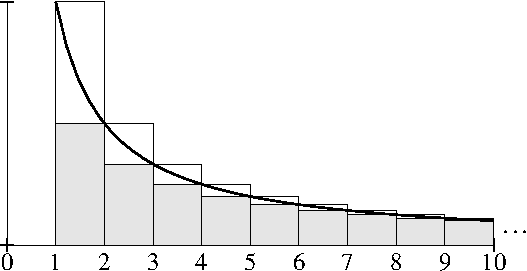
\includegraphics{figures/integraltest}
\caption{The area under the curve, 
$\int_1^\infty f$, is bounded below
by the area of the shaded rectangles,
$f(2)+f(3)+f(4)+\cdots$, and bounded above
by the area entire rectangles,
$f(1)+f(2)+f(3)+\cdots$.\label{fig:integraltest}}
\end{myfigureht}
By \propref{prop:monotoneintegrable},
$f$ is integrable
on every interval $[k,b]$ for all $b > k$, so the statement of the theorem
makes sense without additional hypotheses of integrability.

\begin{proof}
Let $\epsilon > 0$ be given.  And suppose $\int_k^\infty f$ converges.
Let $\ell, m \in \Z$ be such that $m > \ell \geq k$.
Because $f$ is decreasing we have
$\int_{n}^{n+1} f \leq f(n) \leq \int_{n-1}^{n} f$.  Therefore
\begin{equation} \label{impropriemann:eqseries}
\int_\ell^m f
=
\sum_{n=\ell}^{m-1} \int_{n}^{n+1} f
\leq
\sum_{n=\ell}^{m-1} f(n)
\leq
f(\ell) +
\sum_{n=\ell+1}^{m-1} \int_{n-1}^{n} f
\leq
f(\ell)+
\int_\ell^{m-1} f .
\end{equation}
As before, since $f$ is positive then there exists
an $L \in \N$ such that if $\ell \geq L$, then
$\int_\ell^{m} f < \nicefrac{\epsilon}{2}$ for all $m \geq \ell$.
We note 
$f$ must decrease to zero (why?).  So let us also suppose
that for $\ell \geq L$ we have $f(\ell) < \nicefrac{\epsilon}{2}$.
For such $\ell$ and $m$ we have via \eqref{impropriemann:eqseries}
\begin{equation*}
\sum_{n=\ell}^{m} f(n)
\leq
f(\ell)+
\int_\ell^{m} f < \nicefrac{\epsilon}{2} + \nicefrac{\epsilon}{2} = \epsilon .
\end{equation*}
The series is therefore Cauchy and thus converges.  The estimate in the
proposition is obtained by letting $m$ go to infinity in
\eqref{impropriemann:eqseries} with $\ell = k$.

Conversely suppose $\int_k^\infty f$ diverges.  
As $f$ is positive then by
\propref{impropriemann:possimp},
the sequence $\{ \int_k^m f \}_{m=k}^\infty$ diverges to infinity.
Using
\eqref{impropriemann:eqseries} with $\ell = k$ we find
\begin{equation*}
\int_k^m f
\leq
\sum_{n=k}^{m-1} f(n) .
\end{equation*}
As the left hand side goes to infinity as $m \to \infty$, so does the right
hand side.
\end{proof}

\begin{example}
Let us show $\sum_{n=1}^\infty \frac{1}{n^2}$ exists and let us
estimate its sum to within 0.01.  As this series is the $p$-series for
$p=2$, we already know it converges, but we have only very roughly
estimated its sum.

Using fundamental theorem of calculus we find that for $k \in \N$
we have
\begin{equation*}
\int_{k}^\infty \frac{1}{x^2}~dx = \frac{1}{k} .
\end{equation*}
In particular, the series must converge.  But we also have that
\begin{equation*}
\frac{1}{k} = \int_k^\infty \frac{1}{x^2}~dx
\leq
\sum_{n=k}^\infty \frac{1}{n^2}
\leq
\frac{1}{k^2}
+
\int_k^\infty \frac{1}{x^2}~dx
=
\frac{1}{k^2}
+
\frac{1}{k} .
\end{equation*}
Adding the partial sum up to $k-1$ we get
\begin{equation*}
\frac{1}{k} + \sum_{n=1}^{k-1} \frac{1}{n^2}
\leq
\sum_{n=1}^\infty \frac{1}{n^2}
\leq
\frac{1}{k^2}
+
\frac{1}{k} + \sum_{n=1}^{k-1} \frac{1}{n^2} .
\end{equation*}
In other words,
$\nicefrac{1}{k} + \sum_{n=1}^{k-1} \nicefrac{1}{n^2}$ is an estimate for
the sum to within $\nicefrac{1}{k^2}$.  Therefore, if we wish to
find the sum to within 0.01, we note $\nicefrac{1}{{10}^2} = 0.01$.  We
obtain
\begin{equation*}
1.6397\ldots
\approx
\frac{1}{10} + \sum_{n=1}^{9} \frac{1}{n^2}
\leq
\sum_{n=1}^\infty \frac{1}{n^2}
\leq
\frac{1}{100}
+
\frac{1}{10} + \sum_{n=1}^{9} \frac{1}{n^2}
\approx
1.6497\ldots .
\end{equation*}
The actual sum is $\nicefrac{\pi^2}{6} \approx 1.6449\ldots$. 
\end{example}

\subsection{Exercises}

\begin{exercise}
Finish the proof of \propref{impropriemann:ptest}.
\end{exercise}

\begin{exercise}
Find out for which $a \in \R$ does $\sum\limits_{n=1}^\infty e^{an}$ converge.
When the series converges, find an upper bound for the sum.
\end{exercise}

\begin{exercise}
{\ }
\begin{enumerate}[a)]
\item
Estimate $\sum\limits_{n=1}^\infty \frac{1}{n(n+1)}$ correct to within 0.01
using the integral test.
\item
Compute the limit of the series exactly
and compare.  Hint: The sum telescopes.
\end{enumerate}
\end{exercise}

\begin{exercise}
Prove 
\begin{equation*}
\int_{-\infty}^\infty \abs{\operatorname{sinc}(x)}~dx = \infty .
\end{equation*}
Hint: Again, it is enough to show this on just one side.
\end{exercise}

\begin{exercise}
Can you interpret
\begin{equation*}
\int_{-1}^1 \frac{1}{\sqrt{\abs{x}}}~dx
\end{equation*}
as an improper integral?  If so, compute its value.
\end{exercise}

\begin{exercise}
Take $f \colon [0,\infty) \to \R$, Riemann integrable on
every interval $[0,b]$, and such that there exist $M$, $a$, and $T$,
such that $\abs{f(t)} \leq M e^{at}$ for all $t \geq T$.  Show that the
\emph{\myindex{Laplace transform}} of $f$ exists.  That is, for
every $s > a$ the following integral converges:
\begin{equation*}
F(s) := \int_{0}^\infty f(t) e^{-st} ~dt .
\end{equation*}
\end{exercise}

\begin{exercise}
Let $f \colon \R \to \R$ be a Riemann integrable function
on every interval $[a,b]$, and such
that $\int_{-\infty}^\infty \abs{f(x)}~dx < \infty$.  Show that the
\emph{\myindex{Fourier sine and cosine transforms}}
exist.  That is, for every $\omega \geq 0$ the
following integrals converge
\begin{equation*}
F^s(\omega) := \frac{1}{\pi} \int_{-\infty}^\infty f(t) \sin(\omega t) ~dt ,
\qquad
F^c(\omega) := \frac{1}{\pi} \int_{-\infty}^\infty f(t) \cos(\omega t) ~dt .
\end{equation*}
Furthermore, show that $F^s$ and $F^c$ are bounded functions.
\end{exercise}

\begin{exercise}
Suppose $f \colon [0,\infty) \to \R$ is Riemann integrable on every interval
$[0,b]$.  Show that  $\int_0^\infty f$ converges if and only if
for every $\epsilon > 0$ there exists an $M$ such that if $M \leq a < b$
then $\abs{\int_a^b f} < \epsilon$.
\end{exercise}

\begin{exercise}
Suppose $f \colon [0,\infty) \to \R$ is nonnegative and
\emph{decreasing}.  Prove:
\begin{enumerate}[a)]
\item
If $\int_0^\infty f < \infty$, then $\lim\limits_{x\to\infty} f(x) = 0$.
\item
The converse does not hold.
\end{enumerate}
\end{exercise}

\begin{exercise}
Find an example of an \emph{unbounded} continuous function $f \colon
[0,\infty) \to \R$ that is nonnegative and such that $\int_0^\infty f < \infty$.
Note that this means that $\lim_{x\to\infty} f(x)$ does not exist; compare
previous exercise.
Hint: On each interval $[k,k+1]$, $k \in \N$, define a function whose
integral over this interval is less than say $2^{-k}$.
\end{exercise}

\begin{exercise}[More challenging]
Find an example of a function $f \colon [0,\infty) \to \R$ integrable on all
intervals such that $\lim_{n\to\infty} \int_0^n f$ converges as a
limit of a sequence, but such that
$\int_0^\infty f$ does not exist.
Hint: For all $n\in \N$, divide $[n,n+1]$ into two halves.  In one half
make the function negative, on the other make the function positive.
\end{exercise}

\begin{exercise}
Suppose $f \colon [1,\infty) \to \R$ is such that
$g(x) := x^2 f(x)$ is a bounded function. Prove that
$\int_1^\infty f$ converges.
\end{exercise}

\begin{exnote}
It is sometimes desirable to assign a value to integrals that normally
cannot be interpreted as even improper integrals,
e.g.\ $\int_{-1}^1 \nicefrac{1}{x}~dx$.
Suppose $f \colon [a,b] \to \R$ is a function and $a < c < b$,
where $f$ is Riemann integrable on the intervals
$[a,c-\epsilon]$ and $[c+\epsilon,b]$ for all $\epsilon > 0$.
Define
the \emph{\myindex{Cauchy principal value}} of $\int_a^b f$ as
\begin{equation*}
p.v.\!\int_a^b f := \lim_{\epsilon\to 0^+}
\left(
\int_a^{c-\epsilon} f + 
\int_{c+\epsilon}^b f
\right) ,
\end{equation*}
if the limit exists.
\end{exnote}

%\begin{samepage}
\begin{exercise}
{\ }
\begin{enumerate}[a)]
\item
Compute $p.v.\!\int_{-1}^1 \nicefrac{1}{x}~dx$.
\item
Compute
$\lim_{\epsilon\to 0^+}
( \int_{-1}^{-\epsilon} \nicefrac{1}{x}~dx + 
\int_{2\epsilon}^1 \nicefrac{1}{x}~dx )$ and show it is not equal
to the principal value.
\item
Show that if $f$ is integrable on $[a,b]$, then
$p.v.\!\int_a^b f = \int_a^b f$ (for an arbitrary $c \in (a,b)$).
\item
Find an example of an $f$ with a singularity at $c$ as above
such that 
$p.v.\!\int_a^b f$ exists, but the improper integrals
$\int_a^c f$ and $\int_c^b f$ diverge.
\item
Suppose 
$f \colon [-1,1] \to \R$ is continuous.  Show that
$p.v.\!\int_{-1}^1 \frac{f(x)}{x}~dx$ exists.
\end{enumerate}
\end{exercise}
%\end{samepage}

\begin{samepage}
\begin{exercise}
Let $f \colon \R \to \R$ and 
$g \colon \R \to \R$ be continuous functions, where
$g(x) = 0$ for all $x \notin [a,b]$ for some interval $[a,b]$.
\begin{enumerate}[a)]
\item
Show that the
\emph{\myindex{convolution}}
\begin{equation*}
(g * f)(x) := \int_{-\infty}^\infty f(t)g(x-t)~dt 
\end{equation*}
is well-defined for all $x \in \R$.
\item
Suppose $\int_{-\infty}^\infty \abs{f(x)}~dx < \infty$.  Prove that
\begin{equation*}
\lim_{x \to -\infty} (g * f)(x) = 0, \qquad \text{and} \qquad
\lim_{x \to \infty} (g * f)(x) = 0 .
\end{equation*}
\end{enumerate}
\end{exercise}
\end{samepage}
